\documentclass[11pt]{article}
\usepackage[margin=1in]{geometry}
\usepackage{amsmath,amssymb,amsfonts}
\usepackage{graphicx,float,caption,booktabs,enumitem,mathtools,hyperref,helvet}
\renewcommand{\familydefault}{\sfdefault}
\setlength{\parindent}{0in}
\setlength{\parskip}{0.6em}
\graphicspath{{HW3/}}
\title{Homework 3: Time-Stepping Methods for the Heat Equation}
\author{}
\date{}
\begin{document}
\maketitle

\section*{Problem 1: Time-Stepping Convergence}
\textbf{Question.} Solve the two-dimensional heat equation on $[0,2\pi]^2$ up to $T=2\pi$ using Forward Euler (FE), Backward Euler (BE), Crank--Nicolson (CN), second-order Runge--Kutta (RK2), and BDF2. Compare the numerical solutions with the exact solution for $N=64$ and $N=128$, and investigate the convergence order as $\Delta t$ decreases.

\subsection*{Solution}
We solve
\[
 u_t=\nabla^2u+f(x,y,t),\qquad
 u(x,y,0)=\sin x\sin y,
\]
with zero Dirichlet boundary conditions. The exact solution is
\[
 u(x,y,t)=\cos(10t)\sin x\sin y.
\]
Substituting into the heat equation gives
\[
 f(x,y,t)=\bigl(2\cos(10t)-10\sin(10t)\bigr)\sin x\sin y.
\]
After discretizing in space, the equation becomes
\[
 \frac{d\mathbf{u}}{dt}=L\mathbf{u}+\mathbf{f}(t),
\]
where $L$ is the discrete Laplacian. 

I calculated the relative error using
\[
 \mathrm{Err}=\frac{\|\mathbf{u}_{\mathrm{numerical}}(T)-\mathbf{u}_{\mathrm{exact}}(T)\|_2}{\|\mathbf{u}_{\mathrm{exact}}(T)\|_2}.
\]
The expected orders are one for FE and BE, and two for CN, RK2, and BDF2. I estimated the orders from the slopes of the log--log error plots.

Initially, RK2 did not show second-order convergence. Its stable time steps were already so small that the spatial error was larger than the time-stepping error. To better separate the two errors, I changed the spatial discretization from the standard second-order Laplacian to a fourth-order finite-difference approximation:
\[
 u_{xx}(x_i)\approx\frac{-u_{i-2}+16u_{i-1}-30u_i+16u_{i+1}-u_{i+2}}{12h^2}.
\]
I used this approximation in both spatial directions. I also made sure that the explicit methods used time steps within their stability restrictions. With this more accurate spatial discretization, the RK2 method was not dominated by spatial error. The fourth-order Laplacian may be less accurate near the endpoints because the stencil extends beyond the boundaries.

% Replace the filenames below with the actual saved plot filenames.
\begin{figure}[H]
\centering
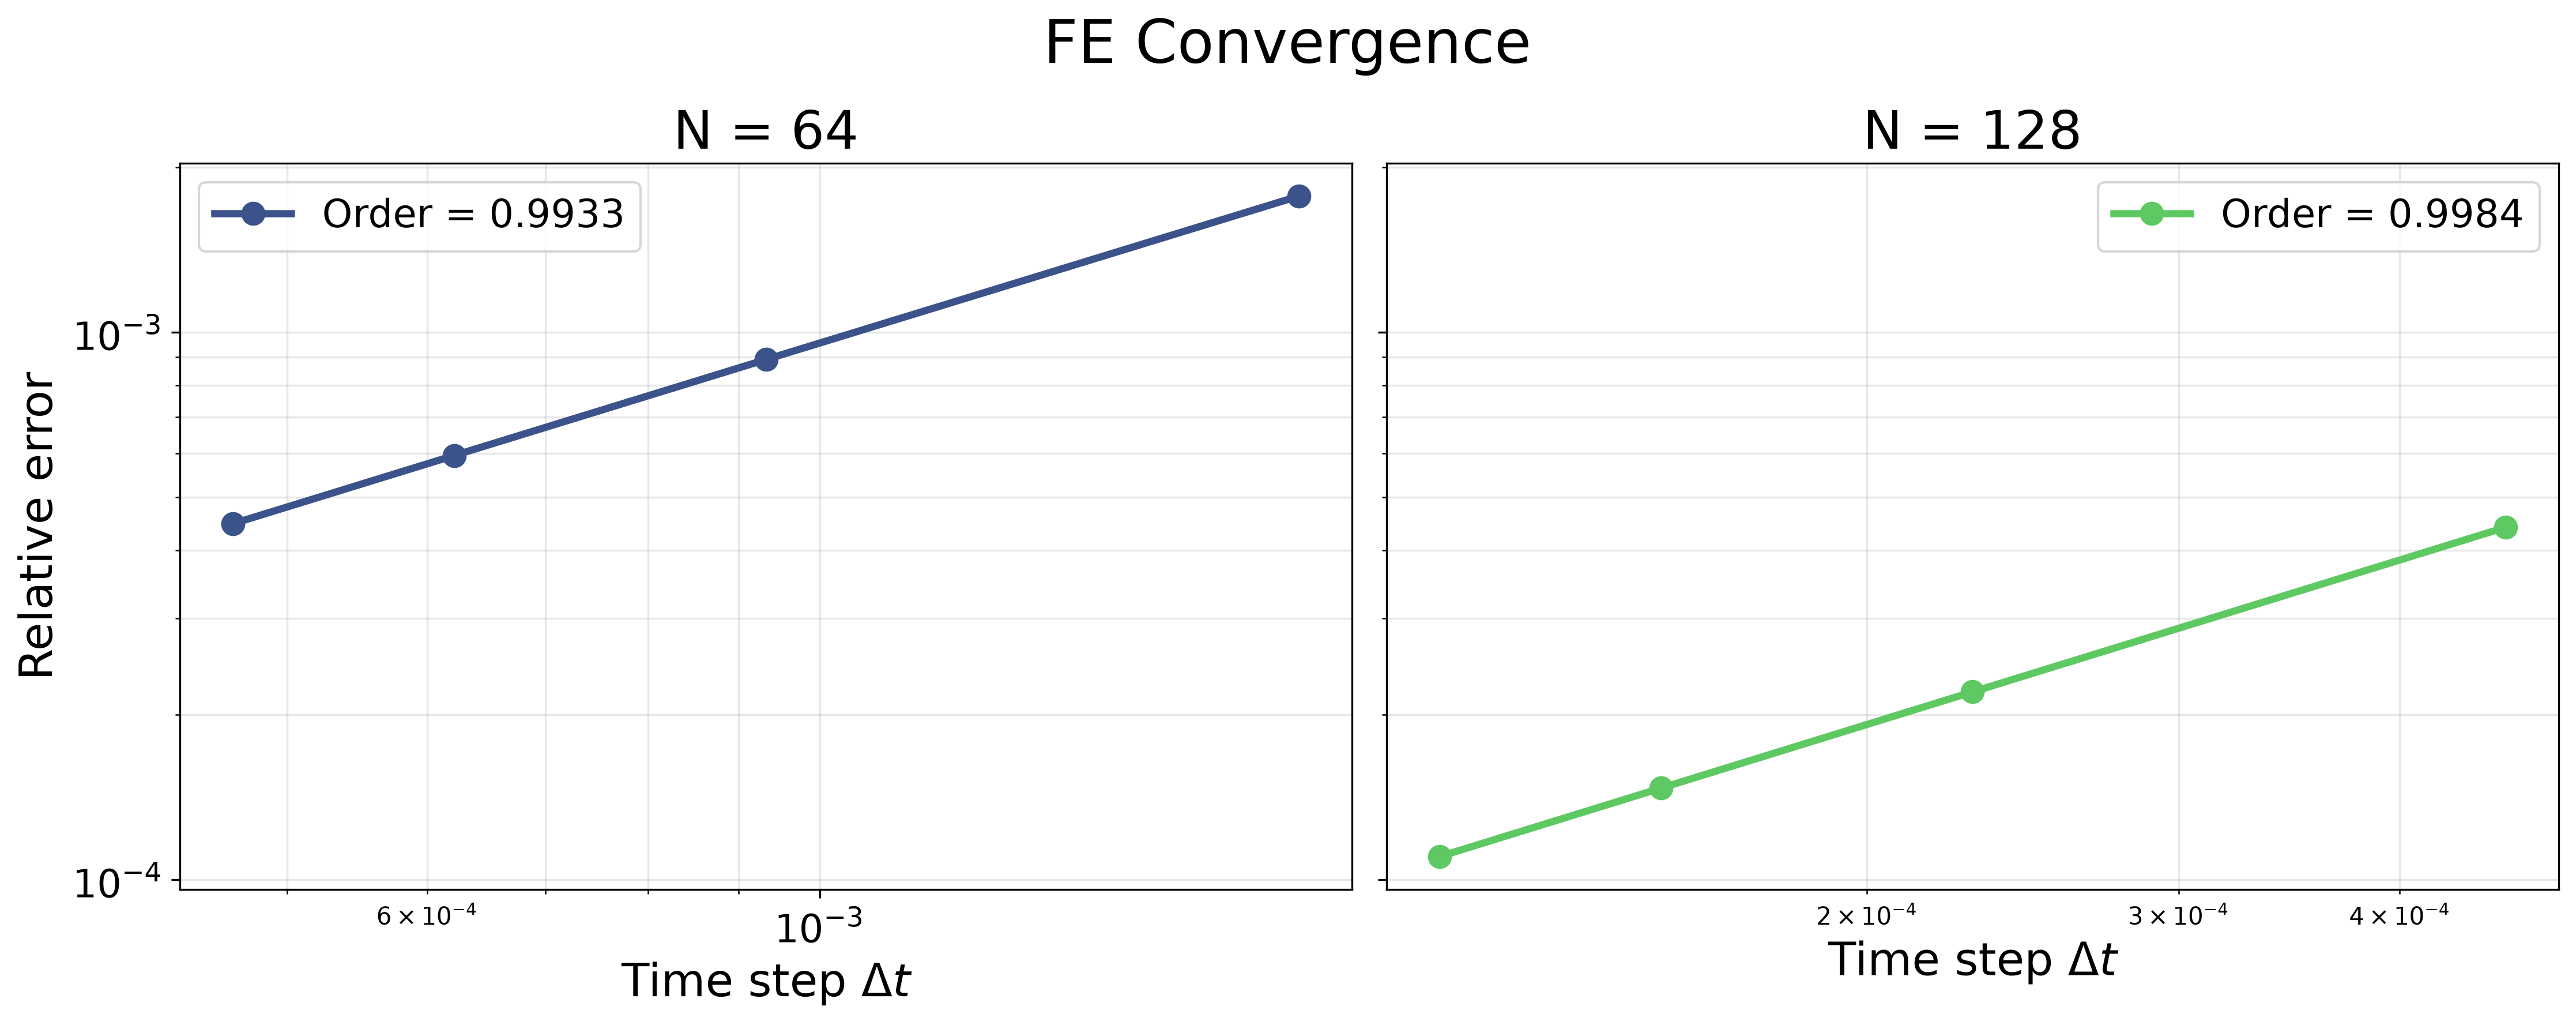
\includegraphics[width=0.95\textwidth]{convergence_FE.png}
\caption{Forward Euler relative error for $N=64$ and $N=128$.}
\end{figure}

\begin{figure}[H]
\centering
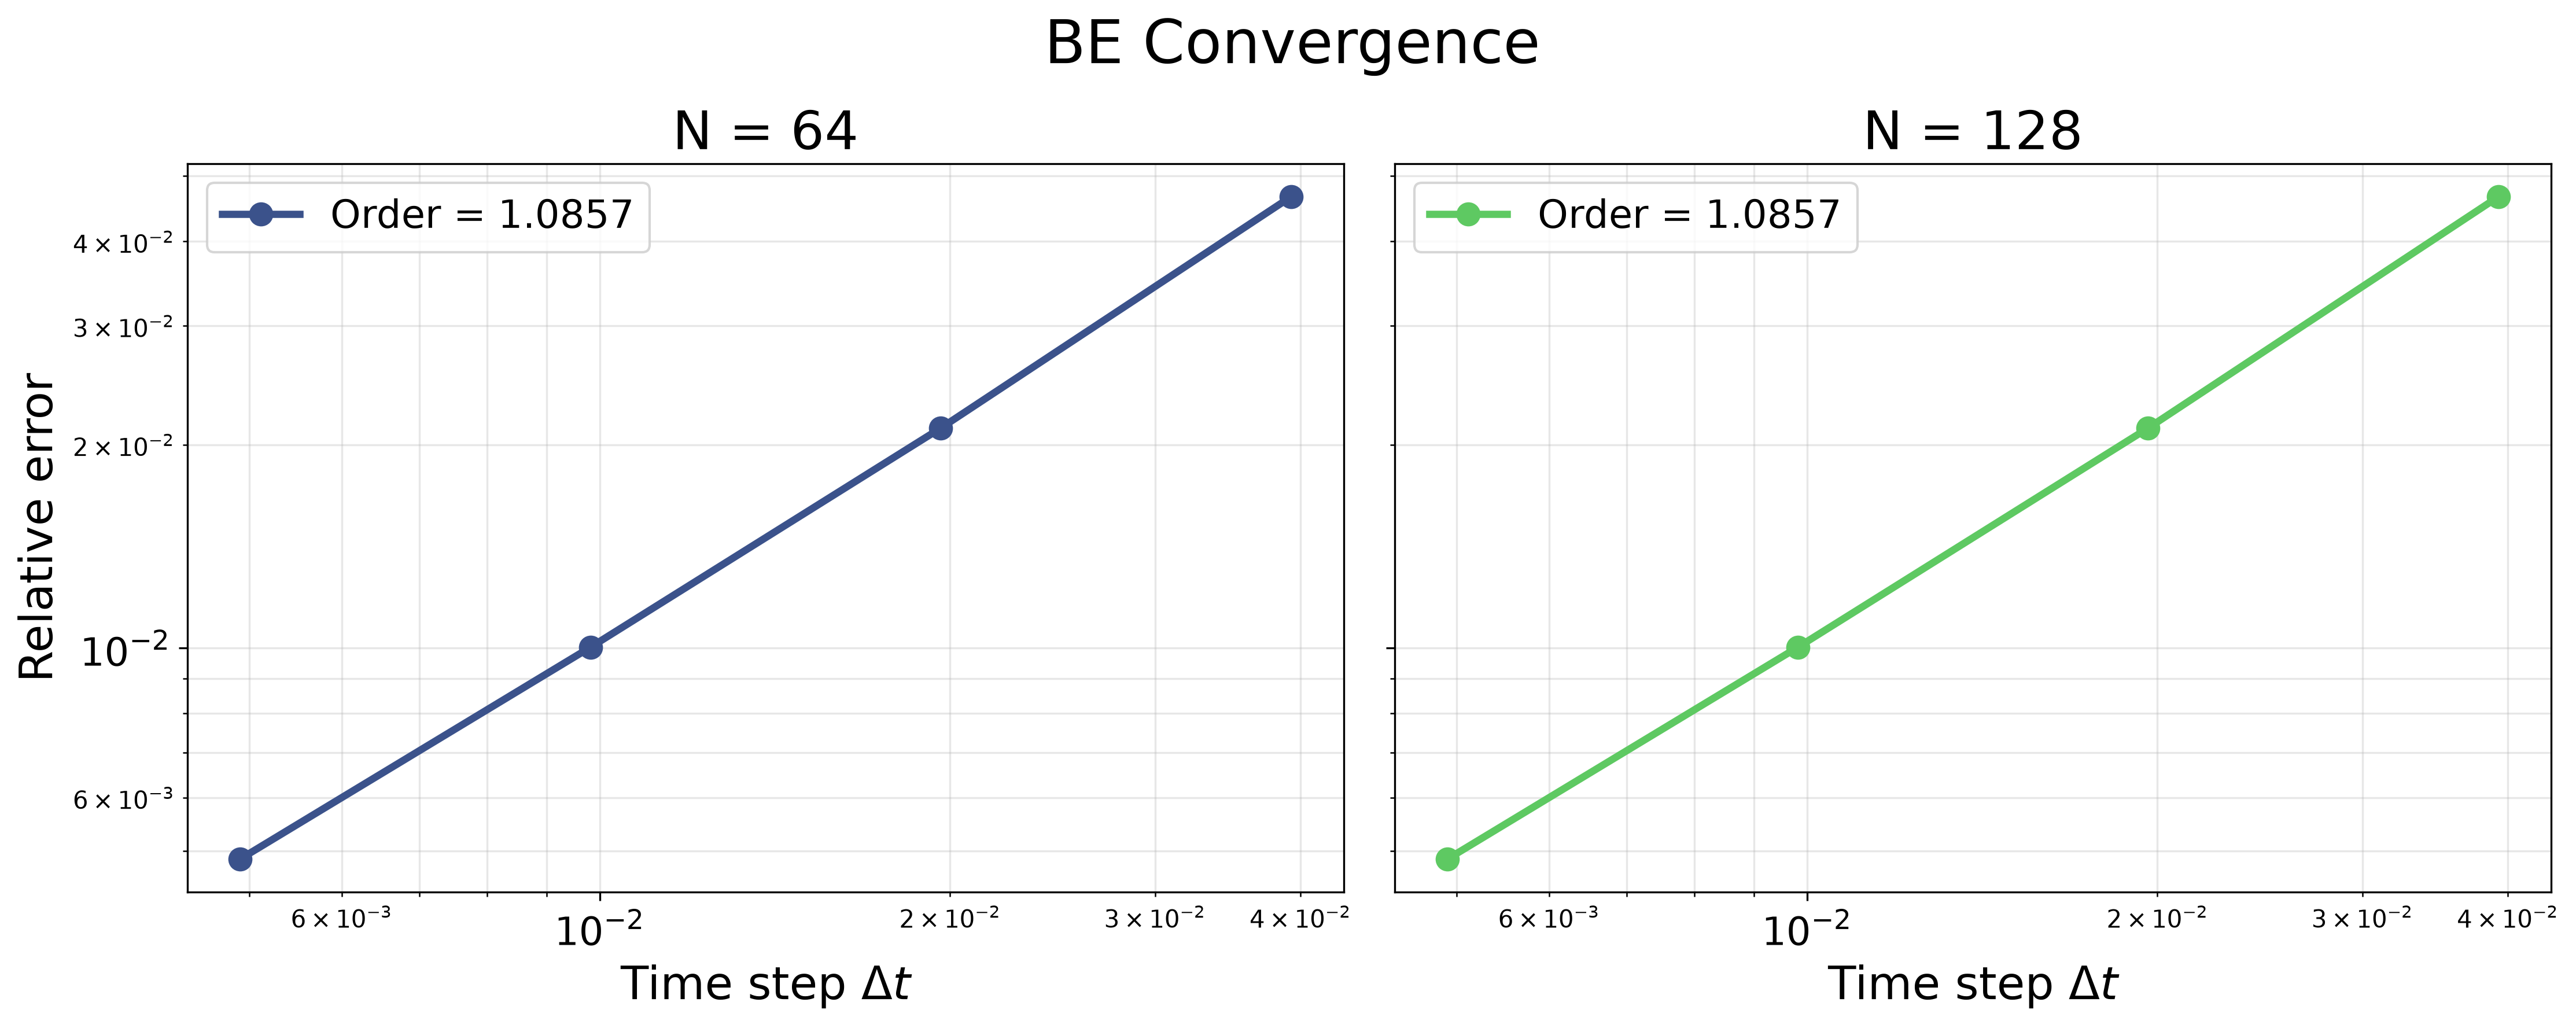
\includegraphics[width=0.95\textwidth]{convergence_BE.png}
\caption{Backward Euler relative error for $N=64$ and $N=128$.}
\end{figure}

\begin{figure}[H]
\centering
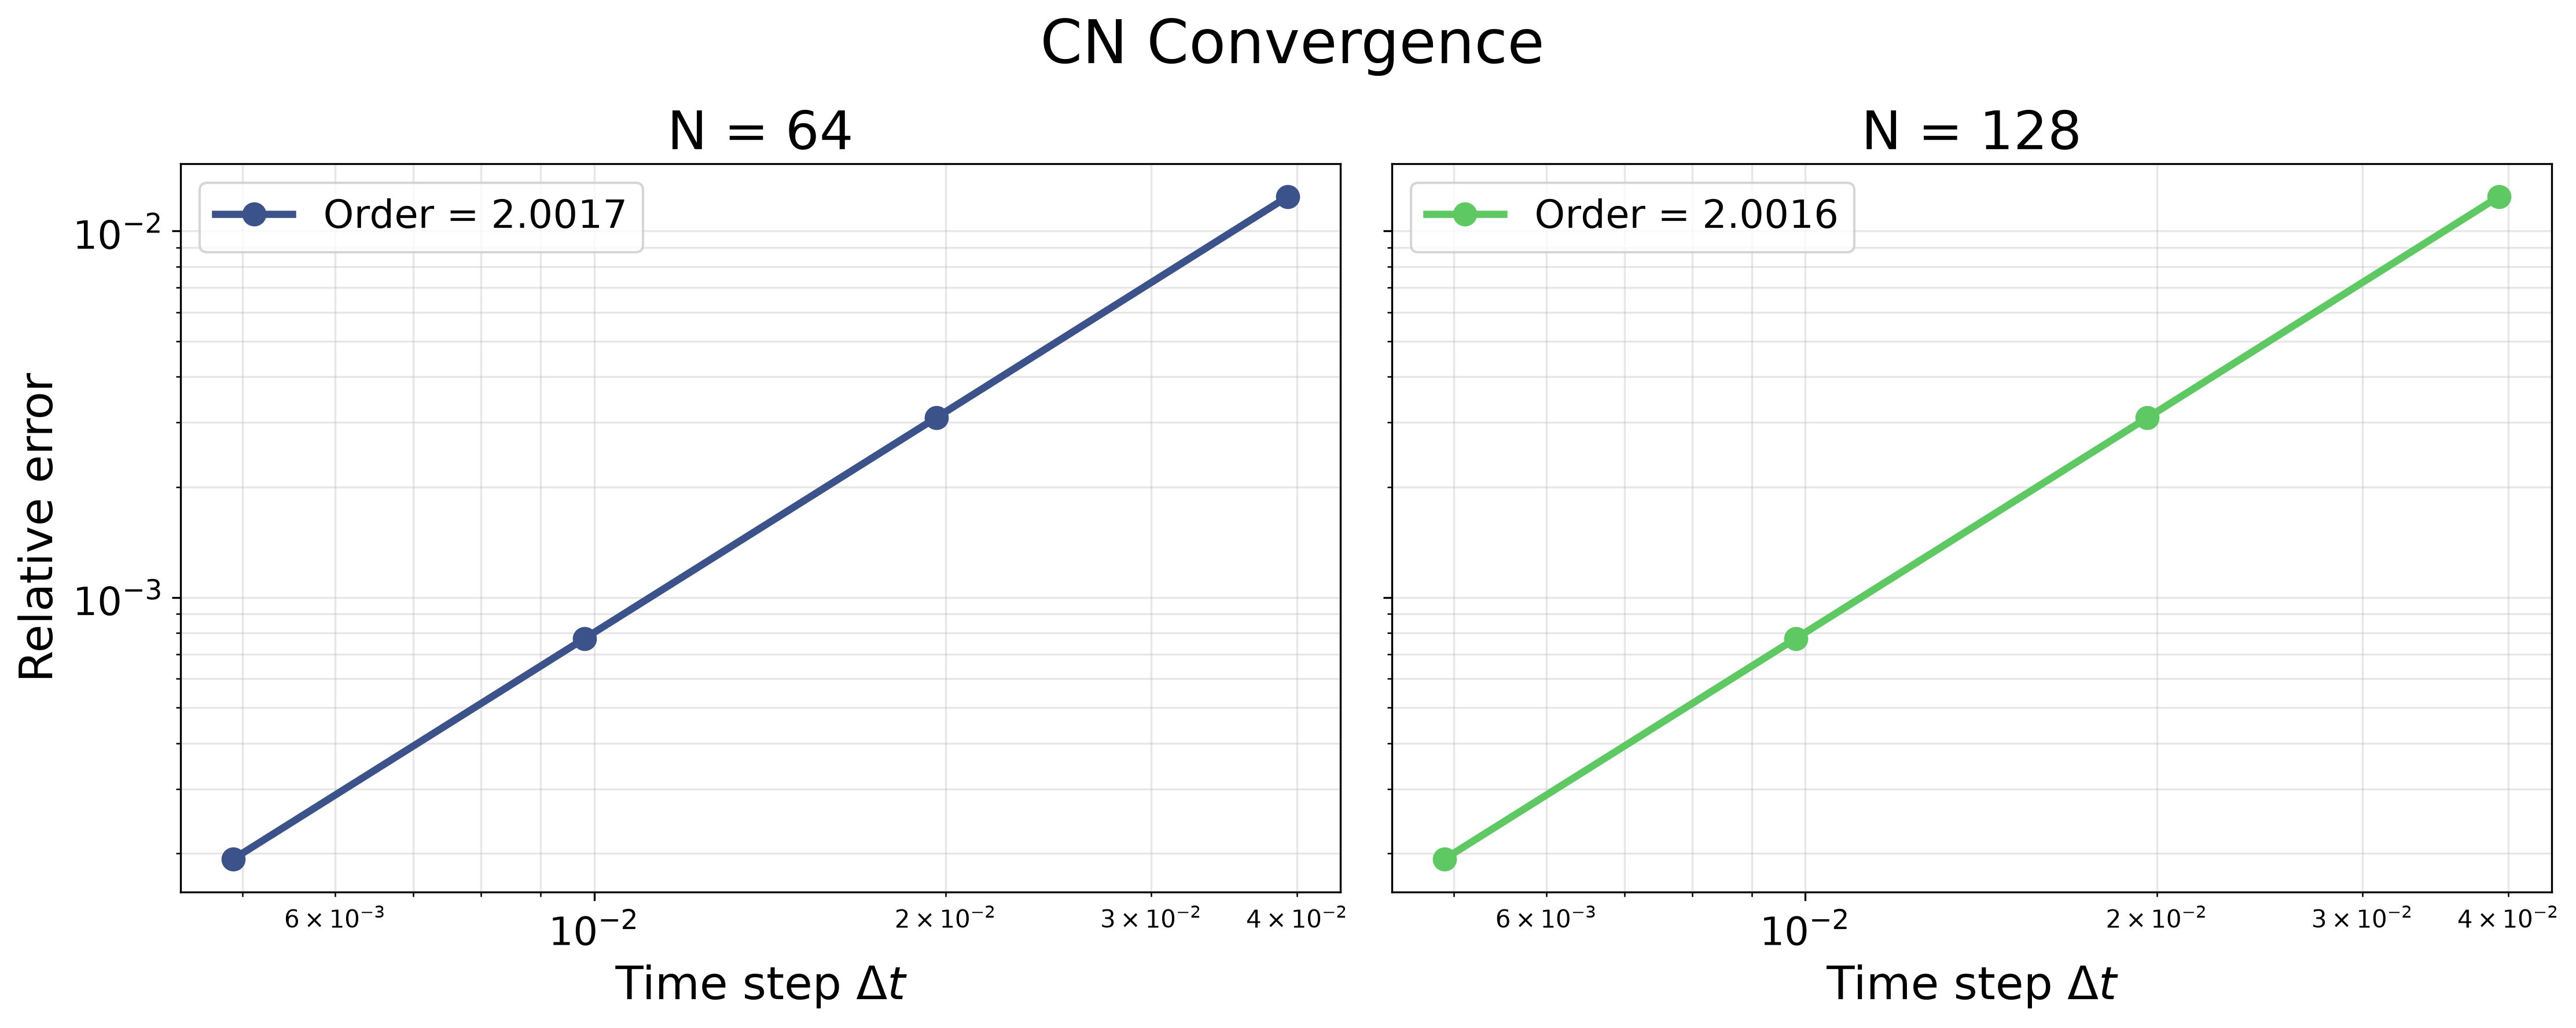
\includegraphics[width=0.95\textwidth]{convergence_CN.png}
\caption{Crank--Nicolson relative error for $N=64$ and $N=128$.}
\end{figure}

\begin{figure}[H]
\centering
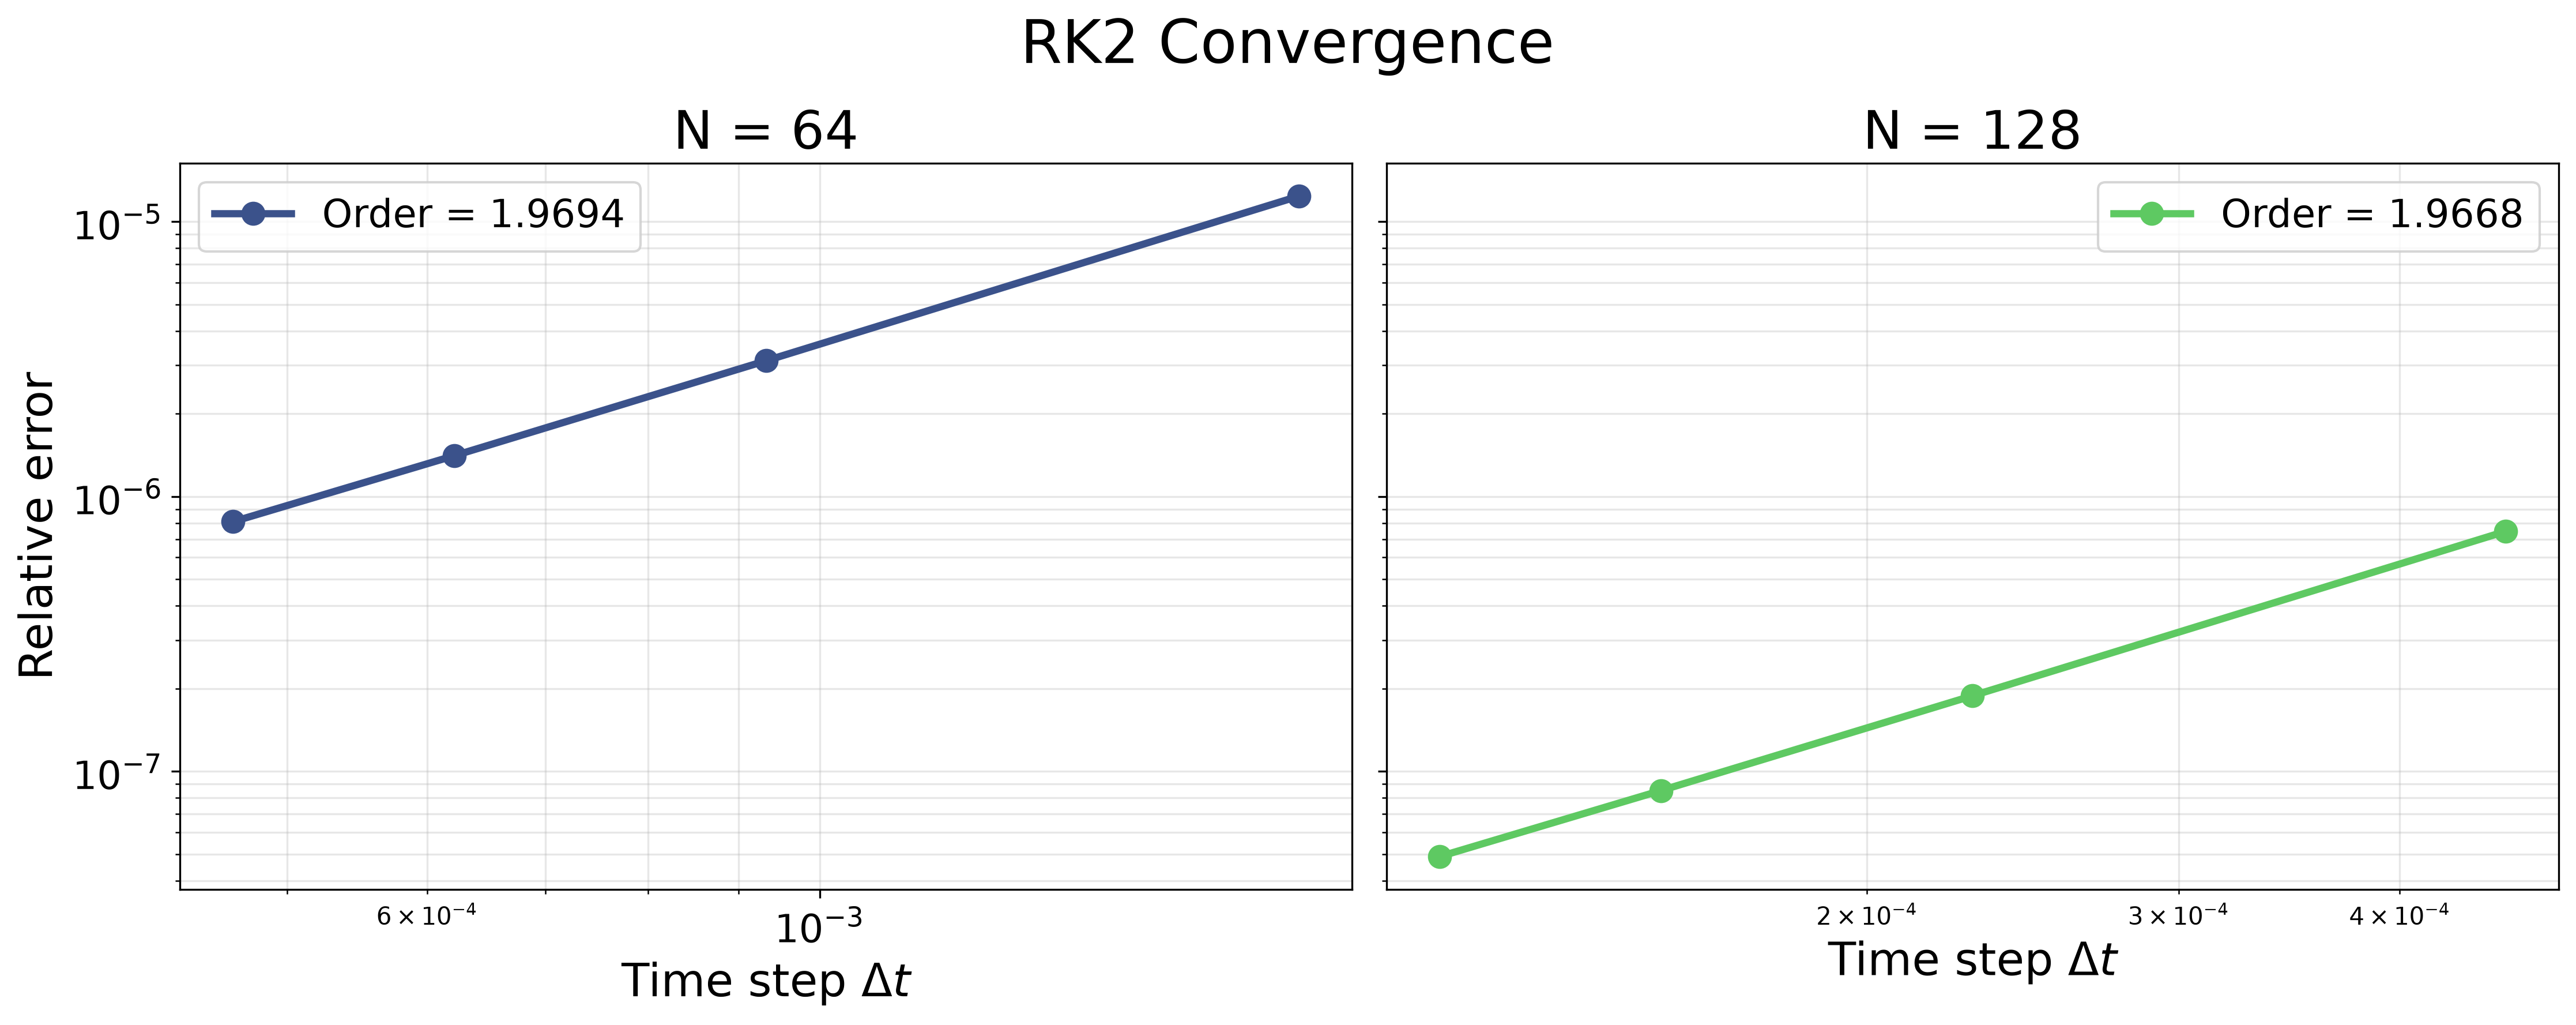
\includegraphics[width=0.95\textwidth]{convergence_RK2.png}
\caption{RK2 relative error for $N=64$ and $N=128$.}
\end{figure}

\begin{figure}[H]
\centering
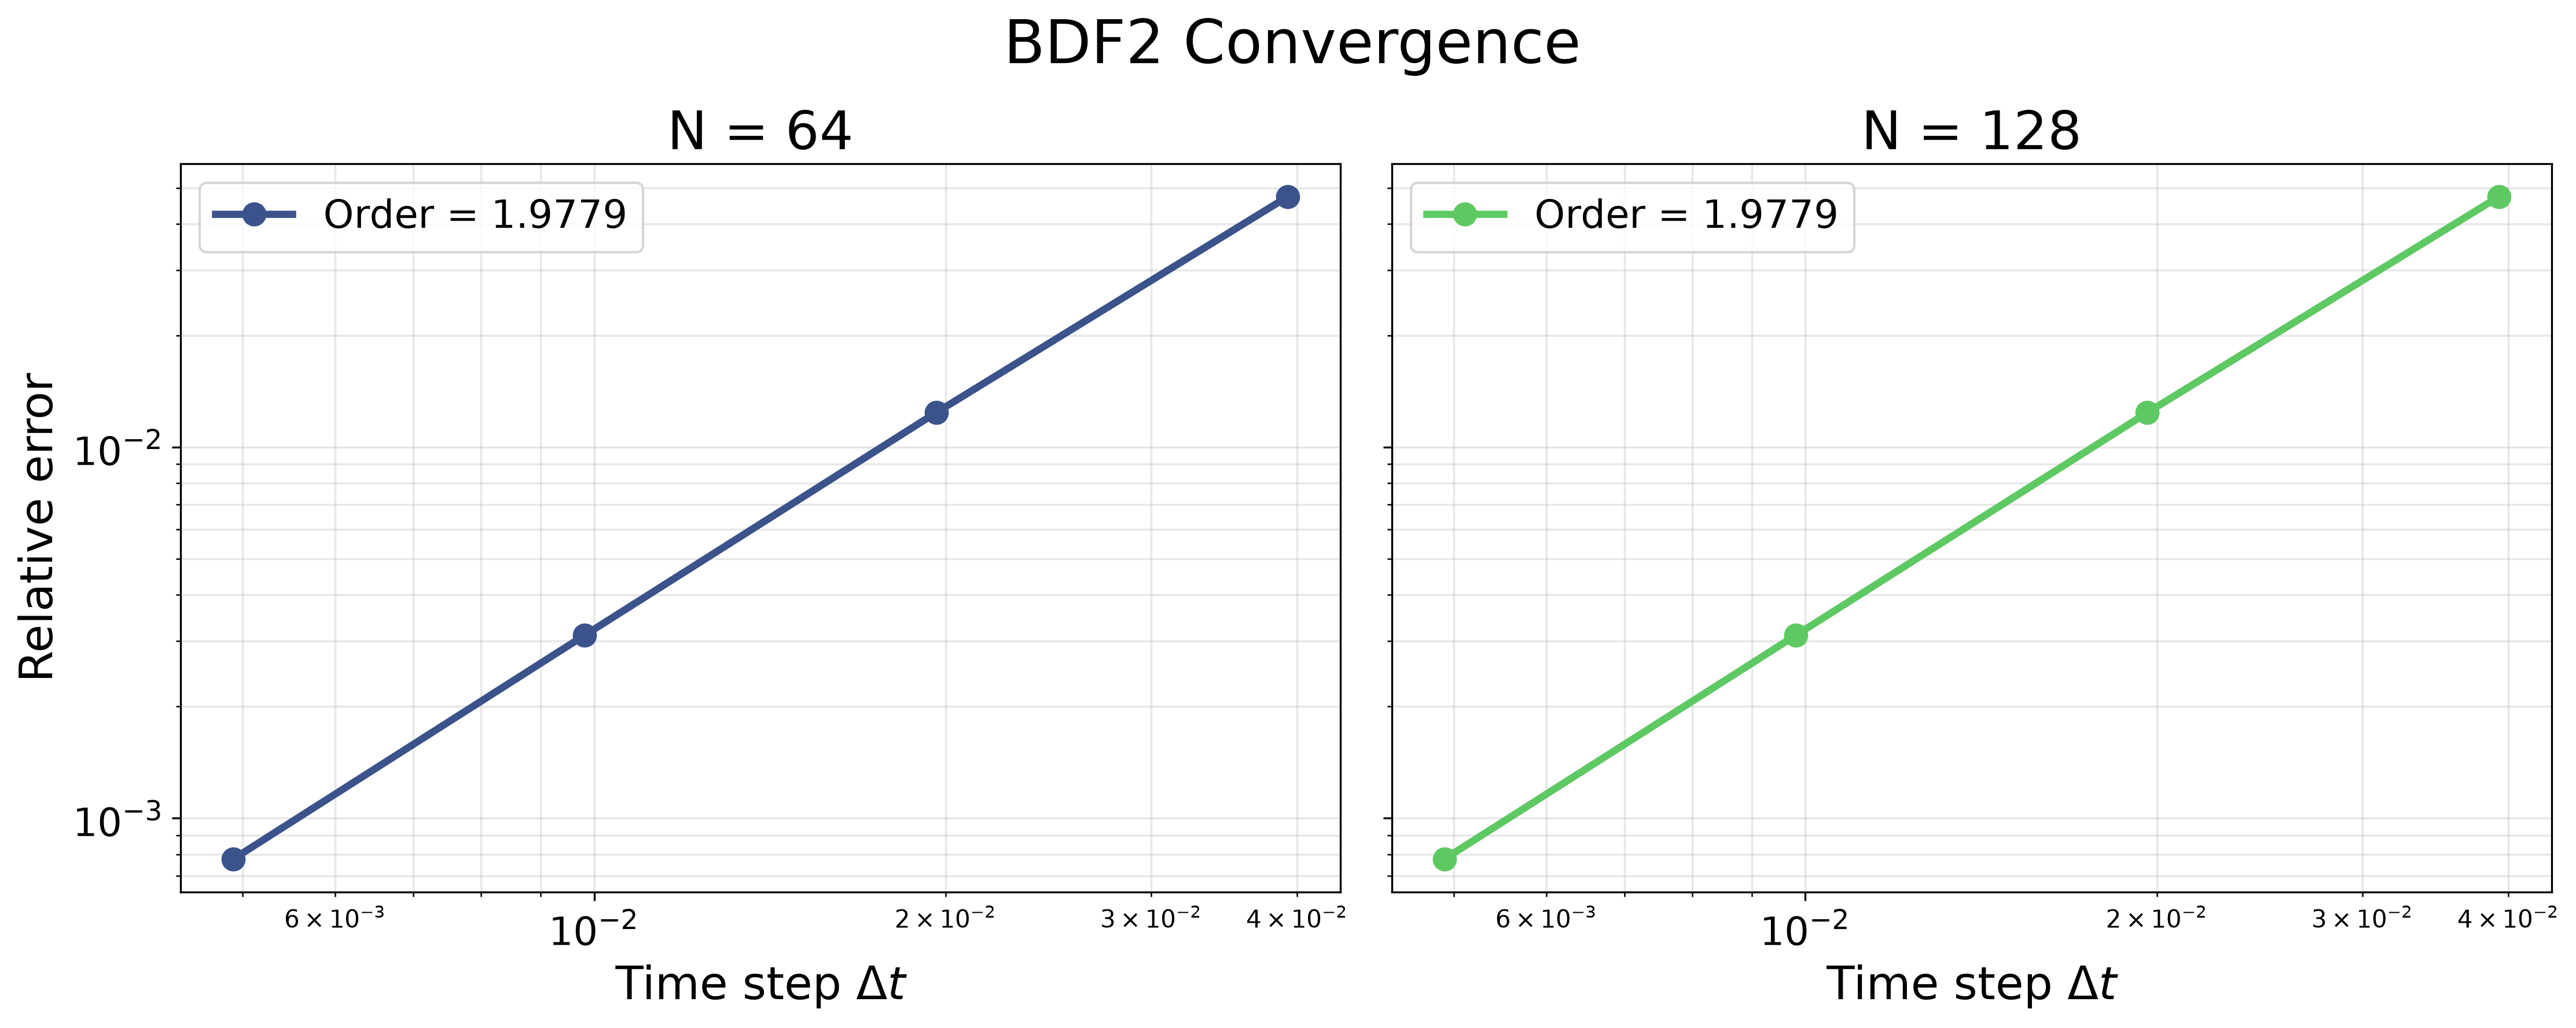
\includegraphics[width=0.95\textwidth]{convergence_BDF2.png}
\caption{BDF2 relative error for $N=64$ and $N=128$.}
\end{figure}

The results generally agree with the expected first-order and second-order behavior over the time-step ranges where temporal error dominates. The error does not decrease indefinitely because spatial discretization also contributes to the total error.

\newpage
\section*{Problem 2: Accuracy and Computational Cost}
\textbf{Question.} For each time-stepping method and for $N=64$ and $N=128$, determine the largest time step that meets relative-error tolerances of $5\times10^{-2}$, $10^{-3}$, and $5\times10^{-6}$. Compare the estimated computational costs and identify the least expensive method for each tolerance that can be reliably met.

\subsection*{Solution}
I compared the relative error against $\Delta t$ and added horizontal lines for the three tolerances. I used the second-order spatial Laplacian for this investigation so that the spatial-error limit would be visible:
\[
 \nabla^2u_{i,j}\approx\frac{u_{i+1,j}+u_{i-1,j}+u_{i,j+1}+u_{i,j-1}-4u_{i,j}}{h^2}.
\]
The total error has contributions from both time and space, which we can summarize as
\[
 \mathrm{Err}=O(\Delta t^p)+O(h^2),
\]
where $p=1$ for FE and BE, and $p=2$ for CN, RK2, and BDF2. This explains why the curves eventually flatten as $\Delta t$ gets smaller. Increasing $N$ reduces the spatial error and lowers the plateau.

For the explicit methods, I restricted $\Delta t$ to the stable range. For the implicit methods, I tested a wider range of time steps. 

\begin{figure}[H]
\centering
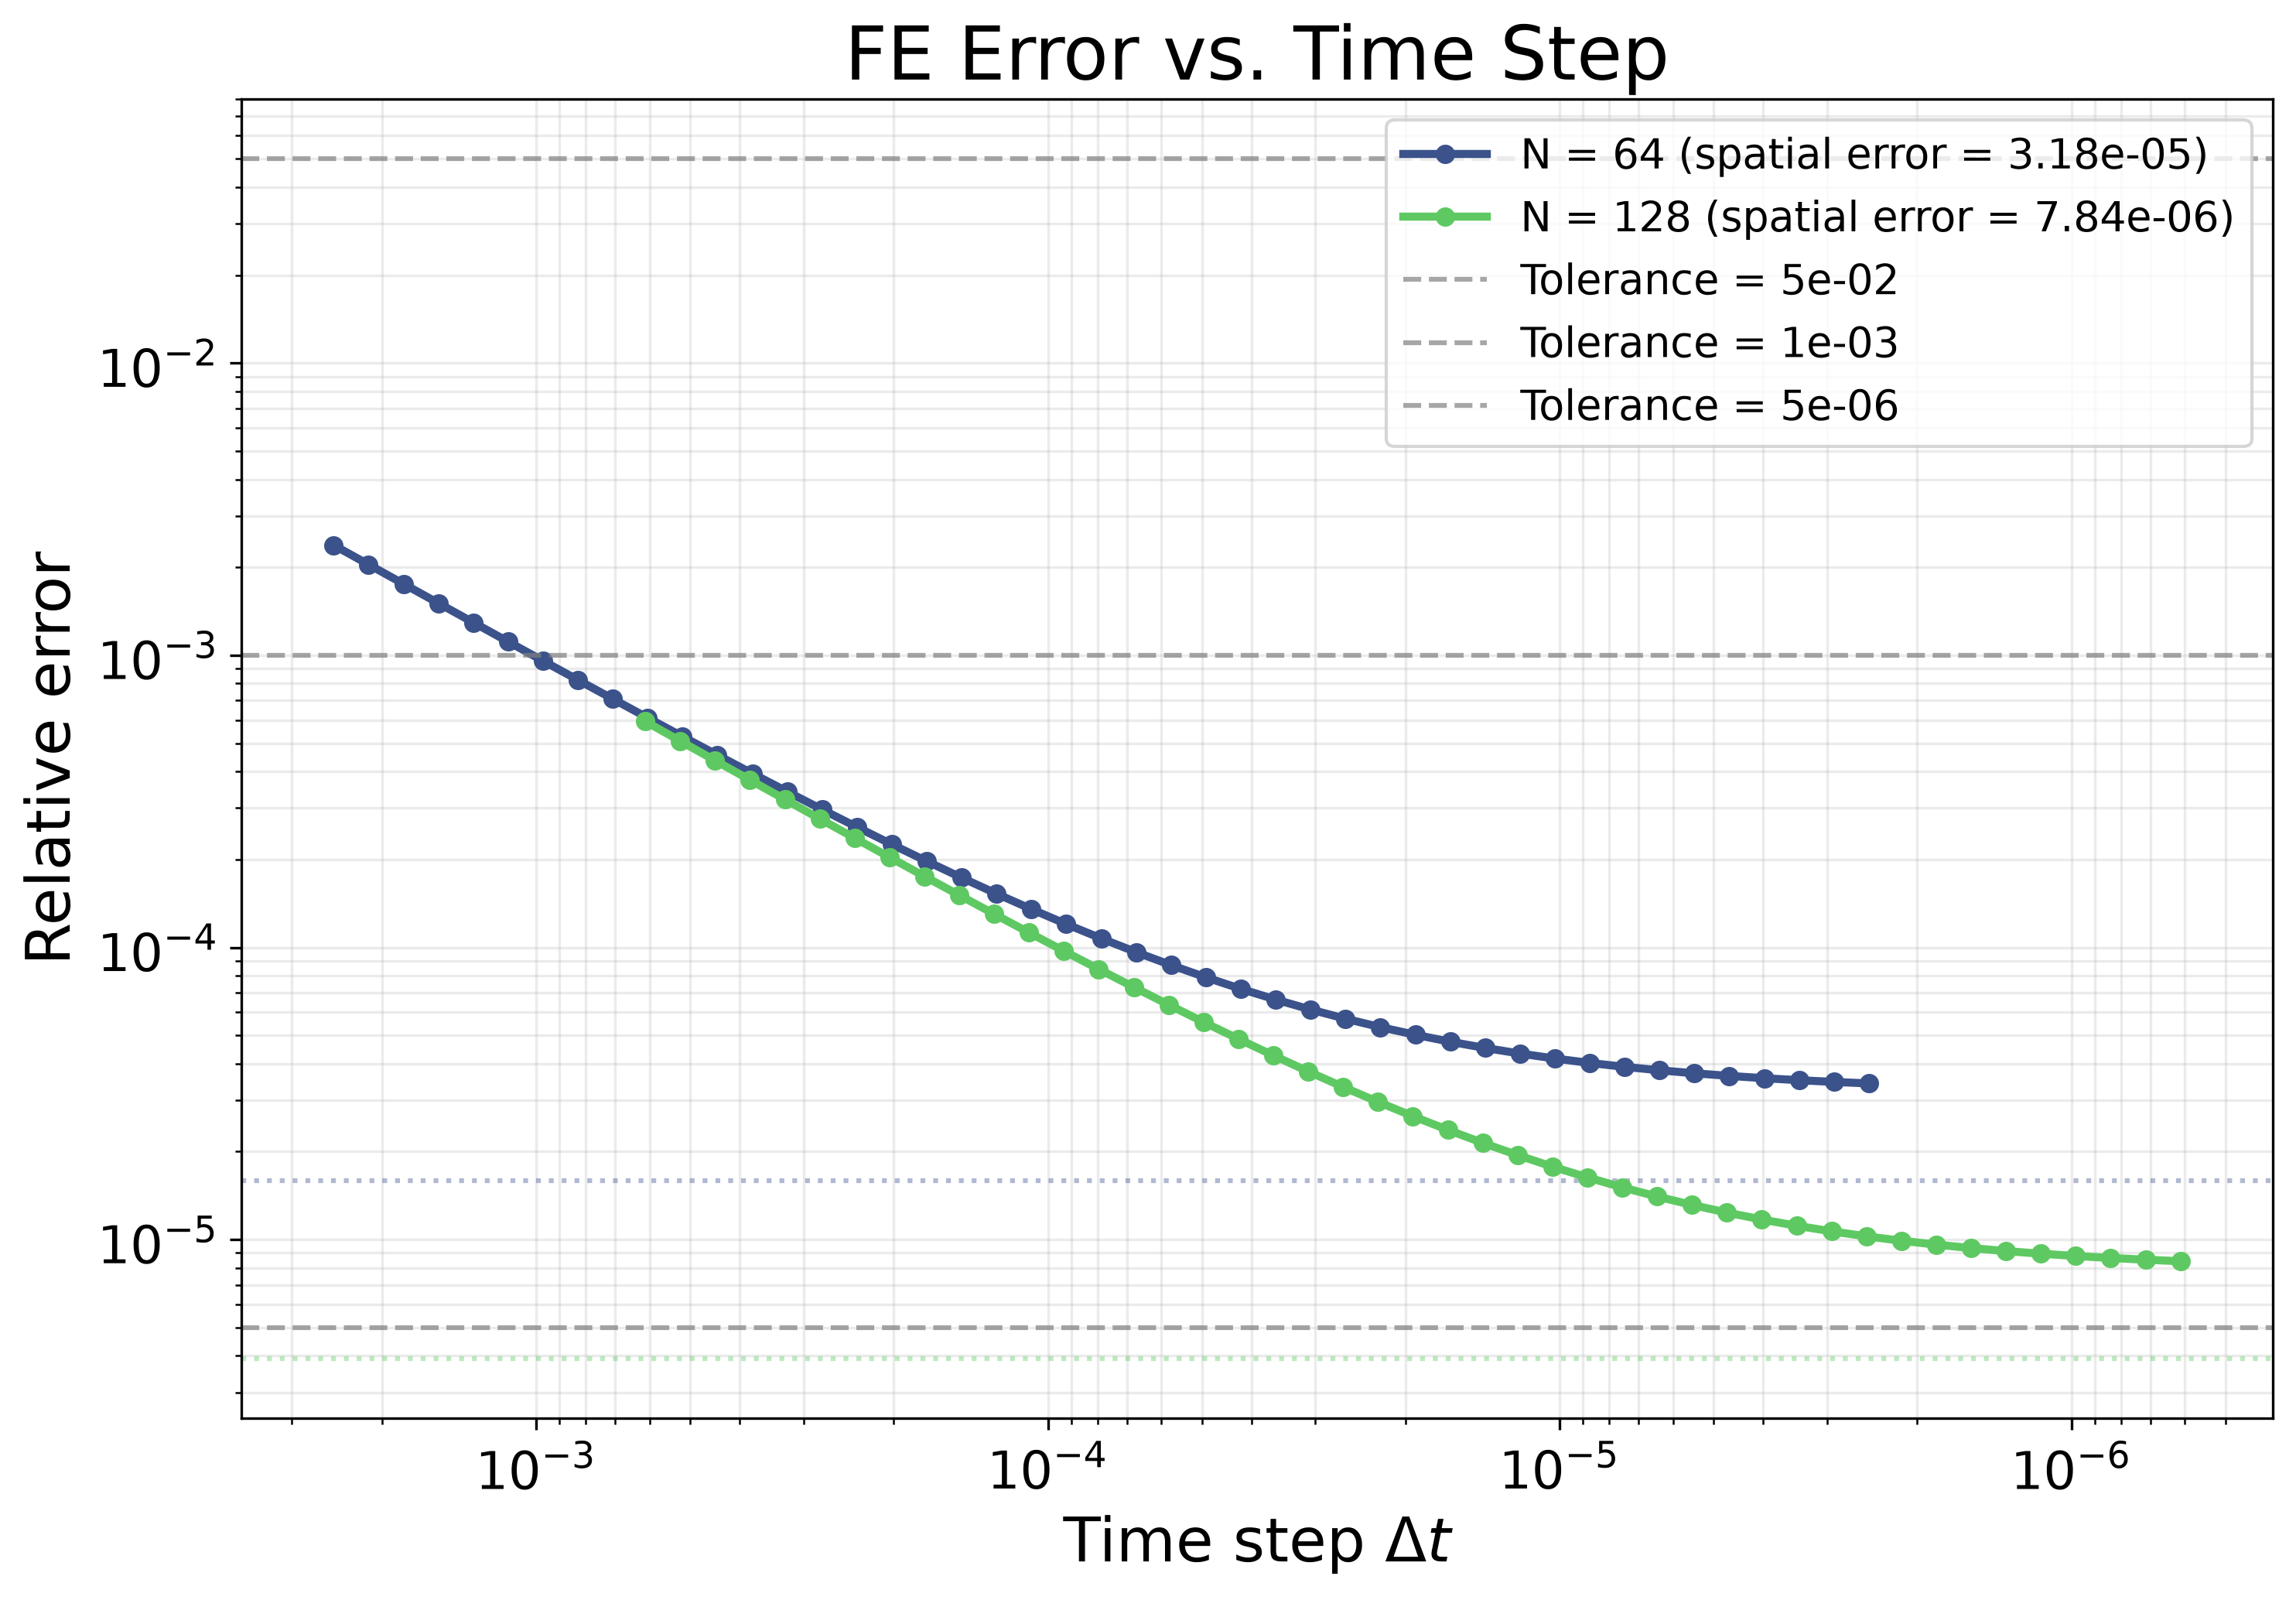
\includegraphics[width=0.8\textwidth]{problem2_FE.png}
\caption{Forward Euler error and the three tolerances.}
\end{figure}

\begin{figure}[H]
\centering
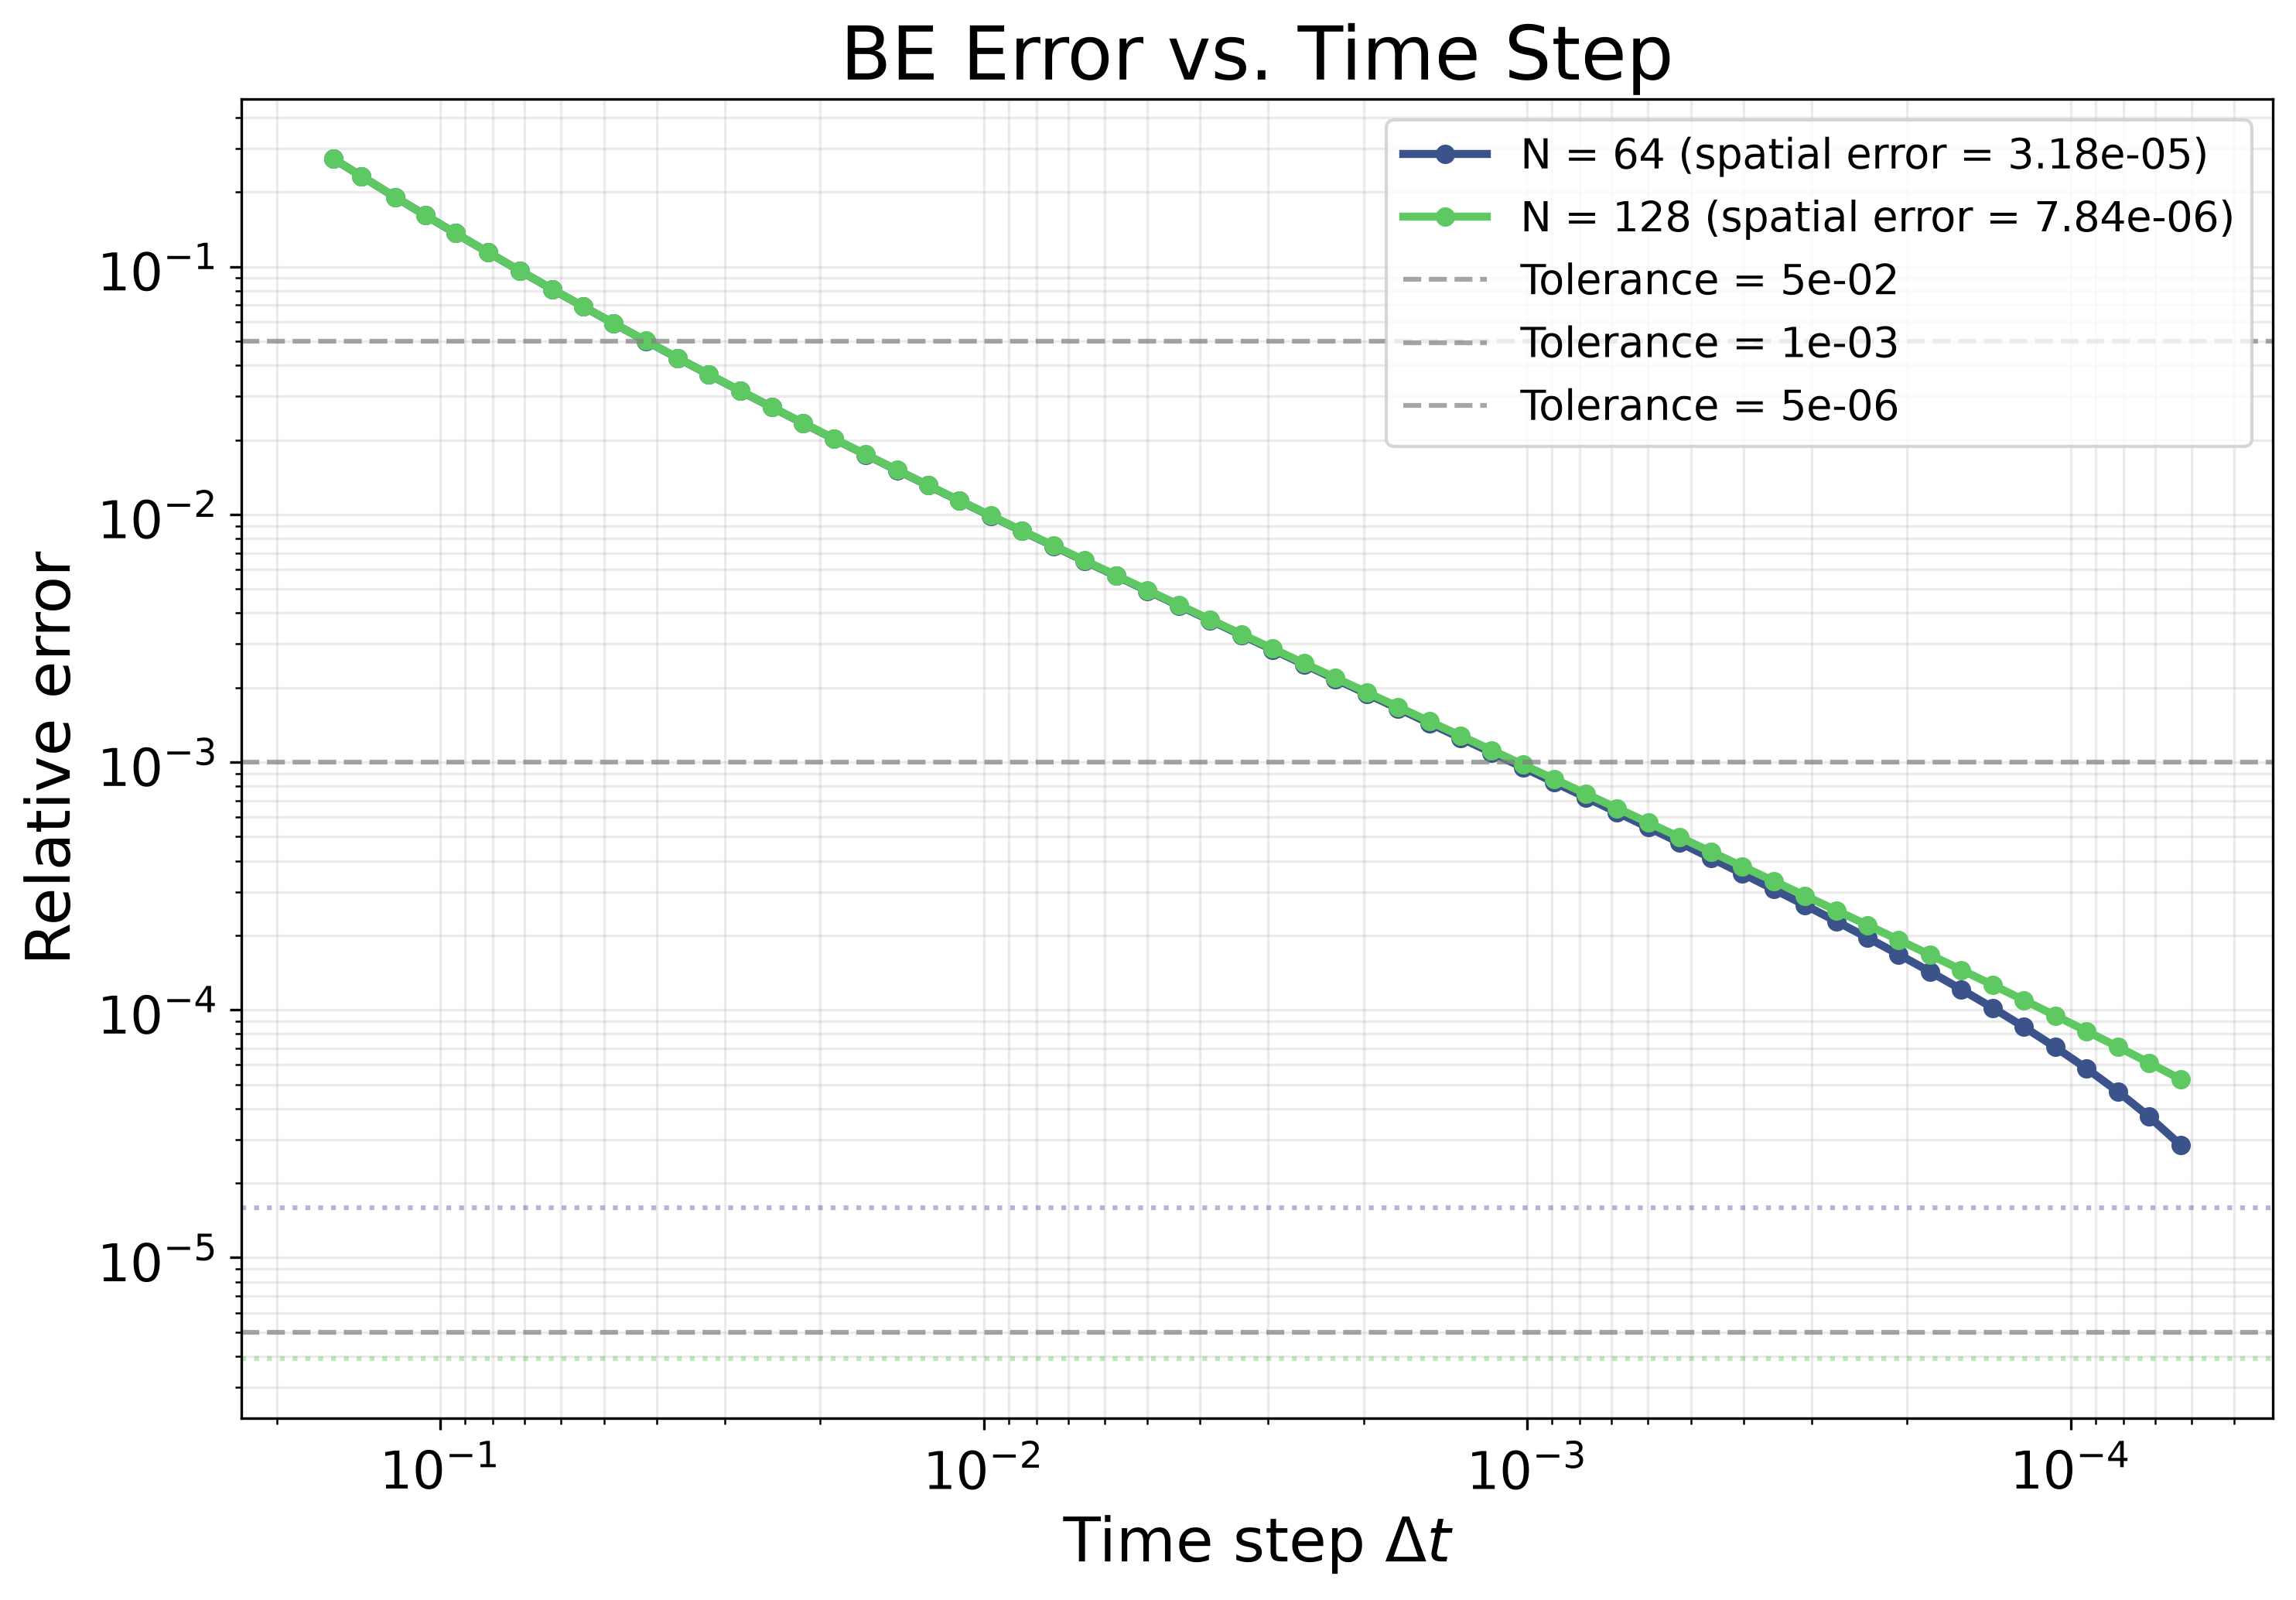
\includegraphics[width=0.8\textwidth]{problem2_BE.png}
\caption{Backward Euler error and the three tolerances.}
\end{figure}

\begin{figure}[H]
\centering
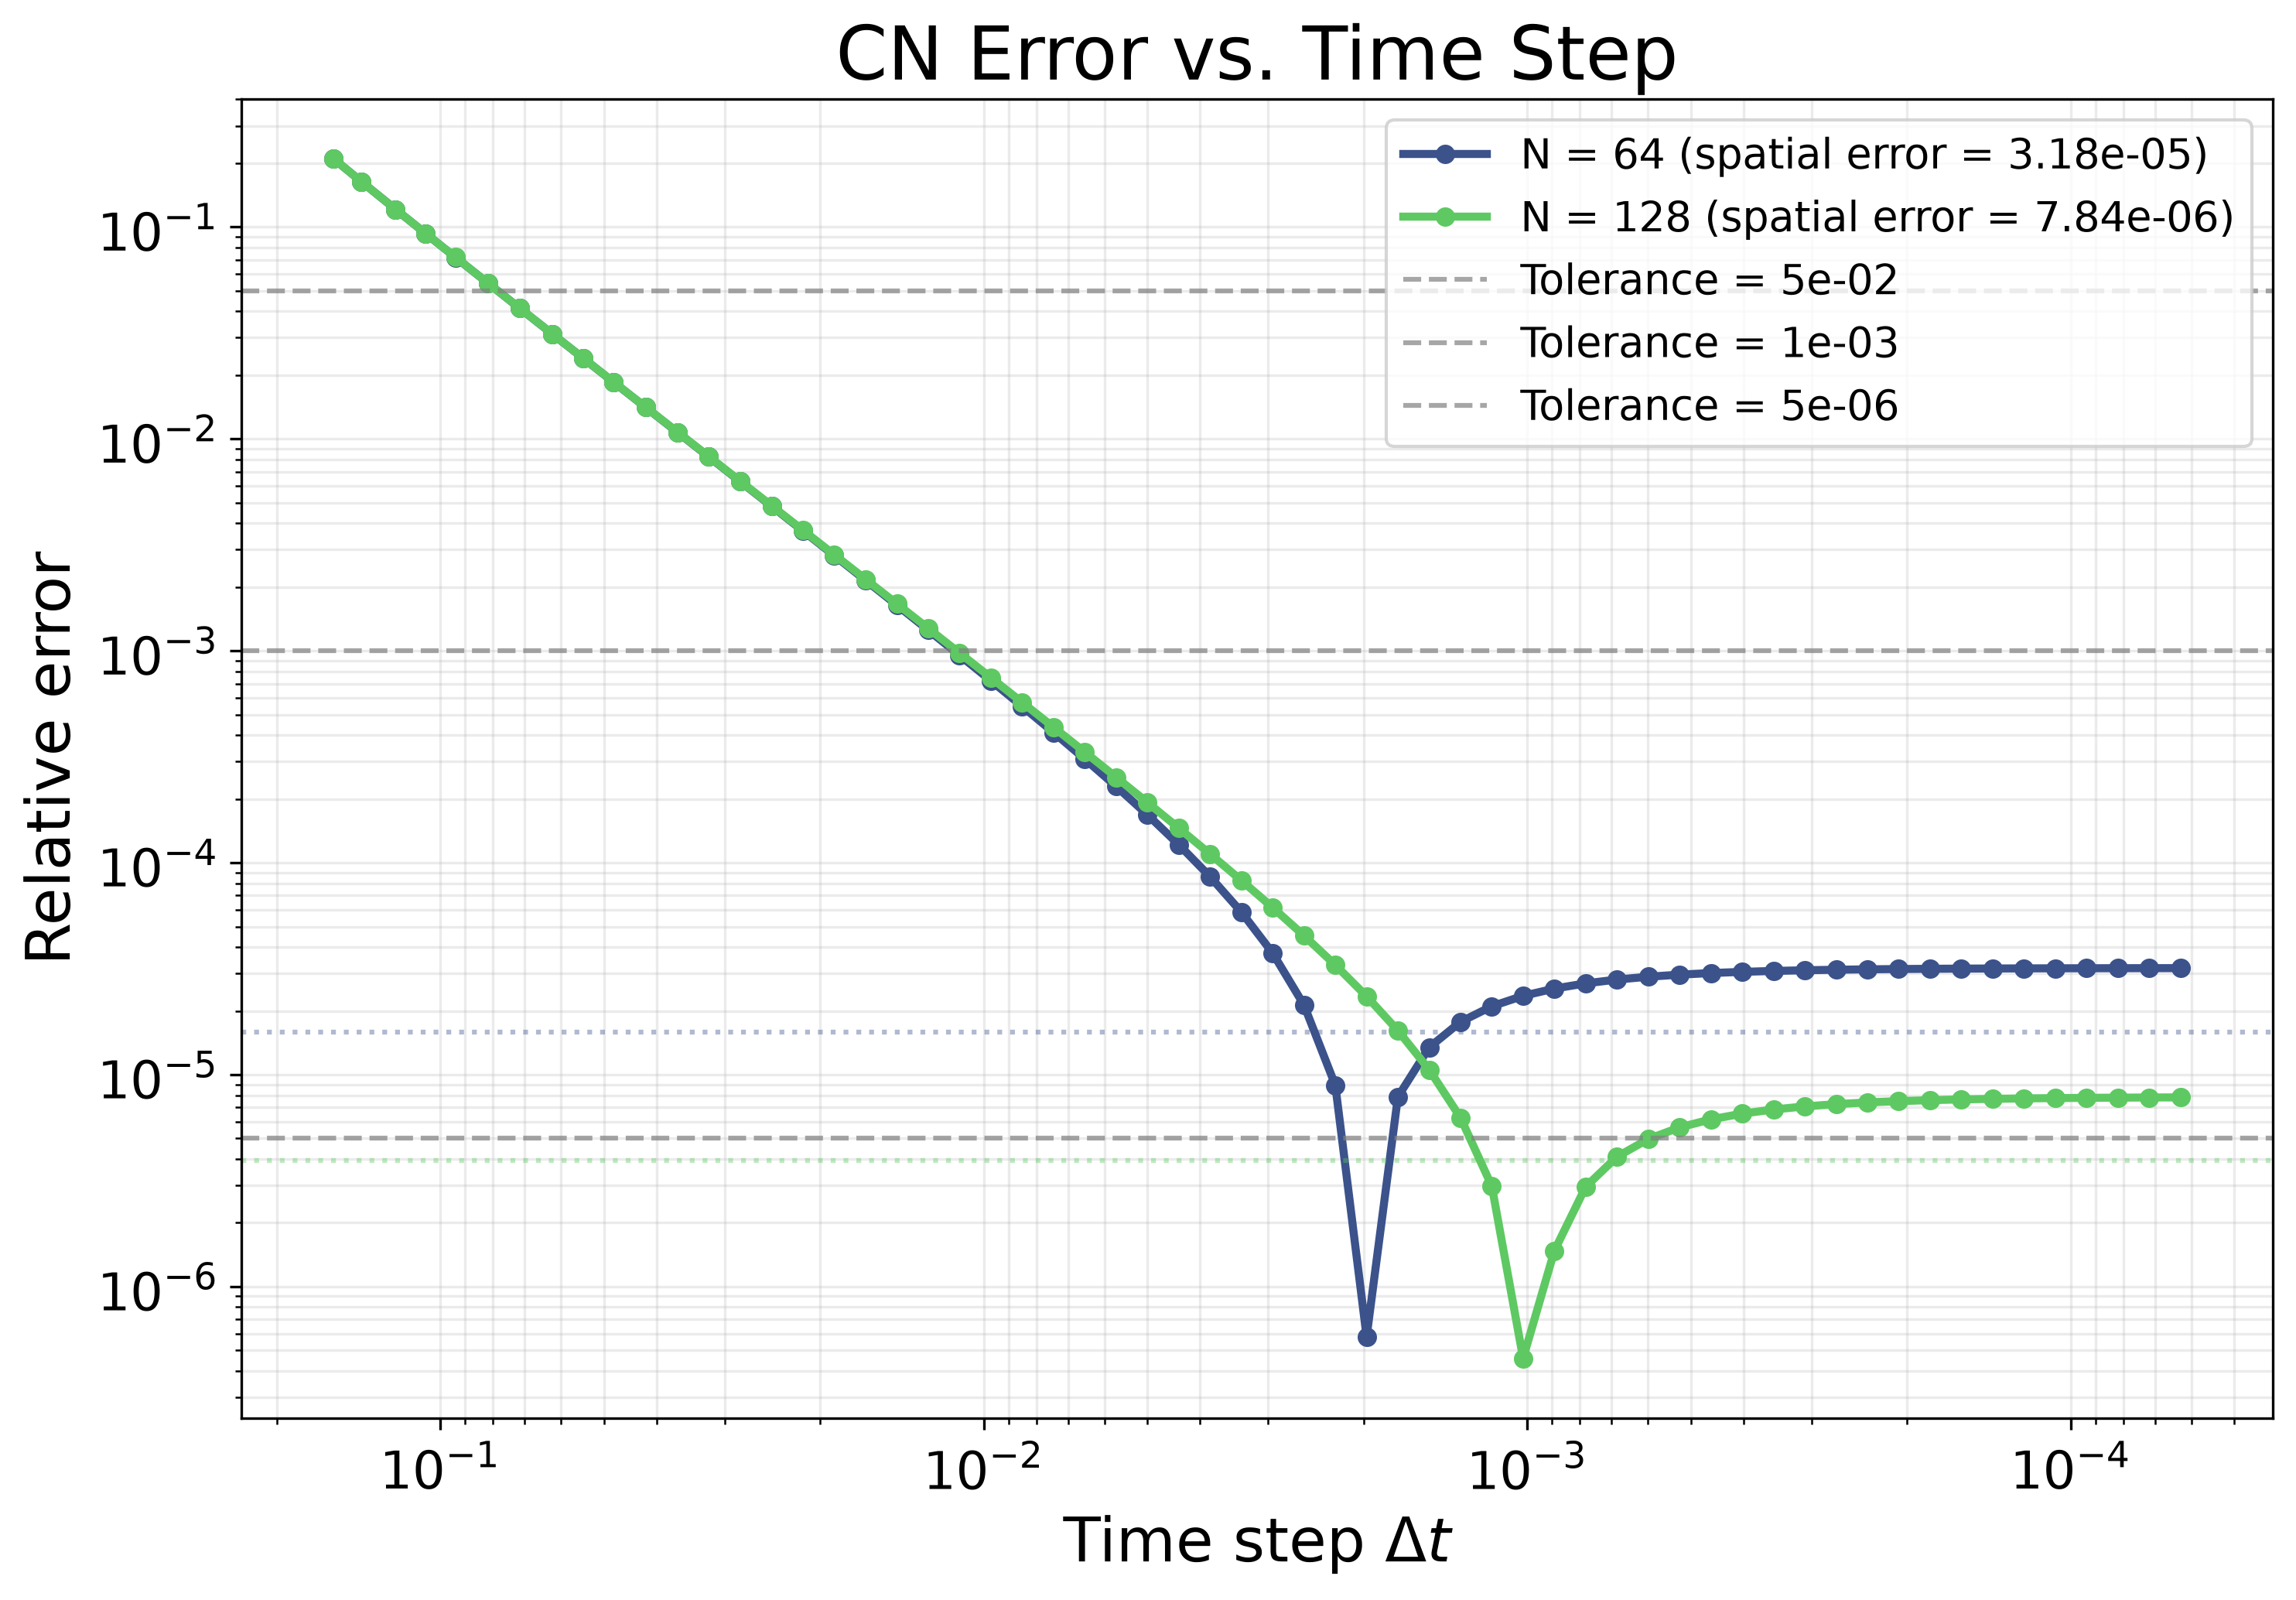
\includegraphics[width=0.8\textwidth]{problem2_CN.png}
\caption{Crank--Nicolson error and the three tolerances.}
\end{figure}

\begin{figure}[H]
\centering
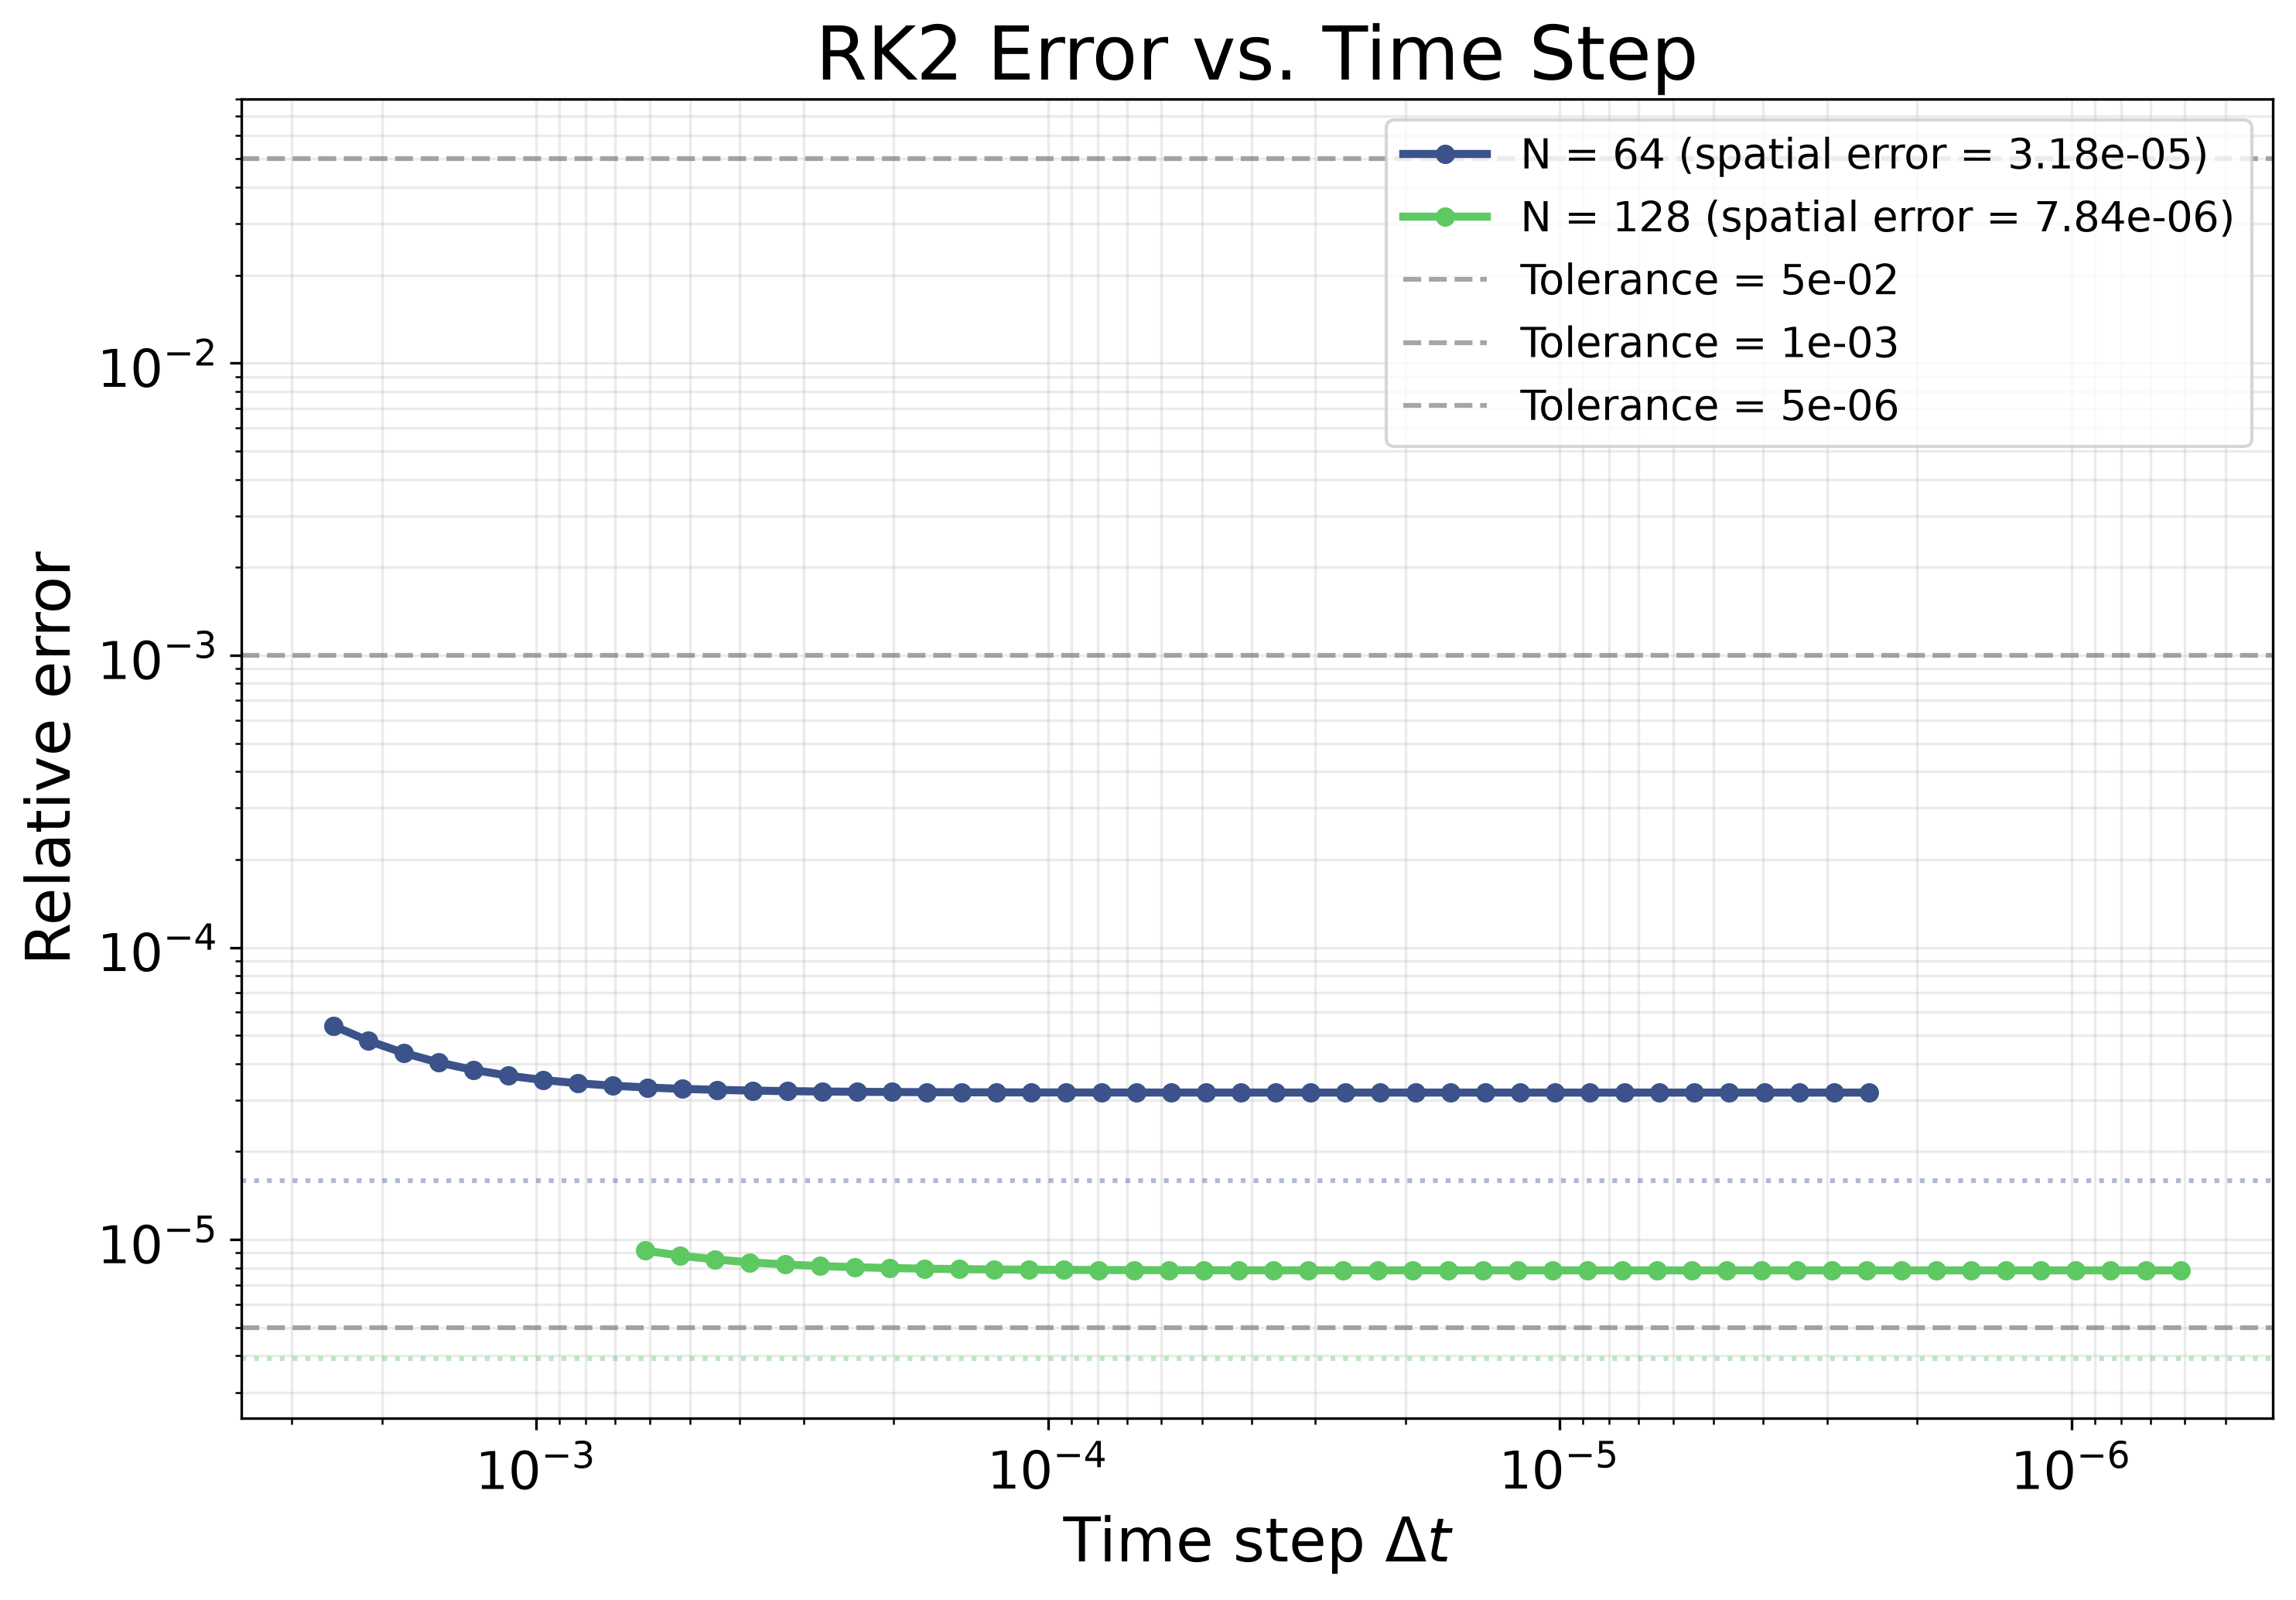
\includegraphics[width=0.8\textwidth]{problem2_RK2.png}
\caption{RK2 error and the three tolerances.}
\end{figure}

\begin{figure}[H]
\centering
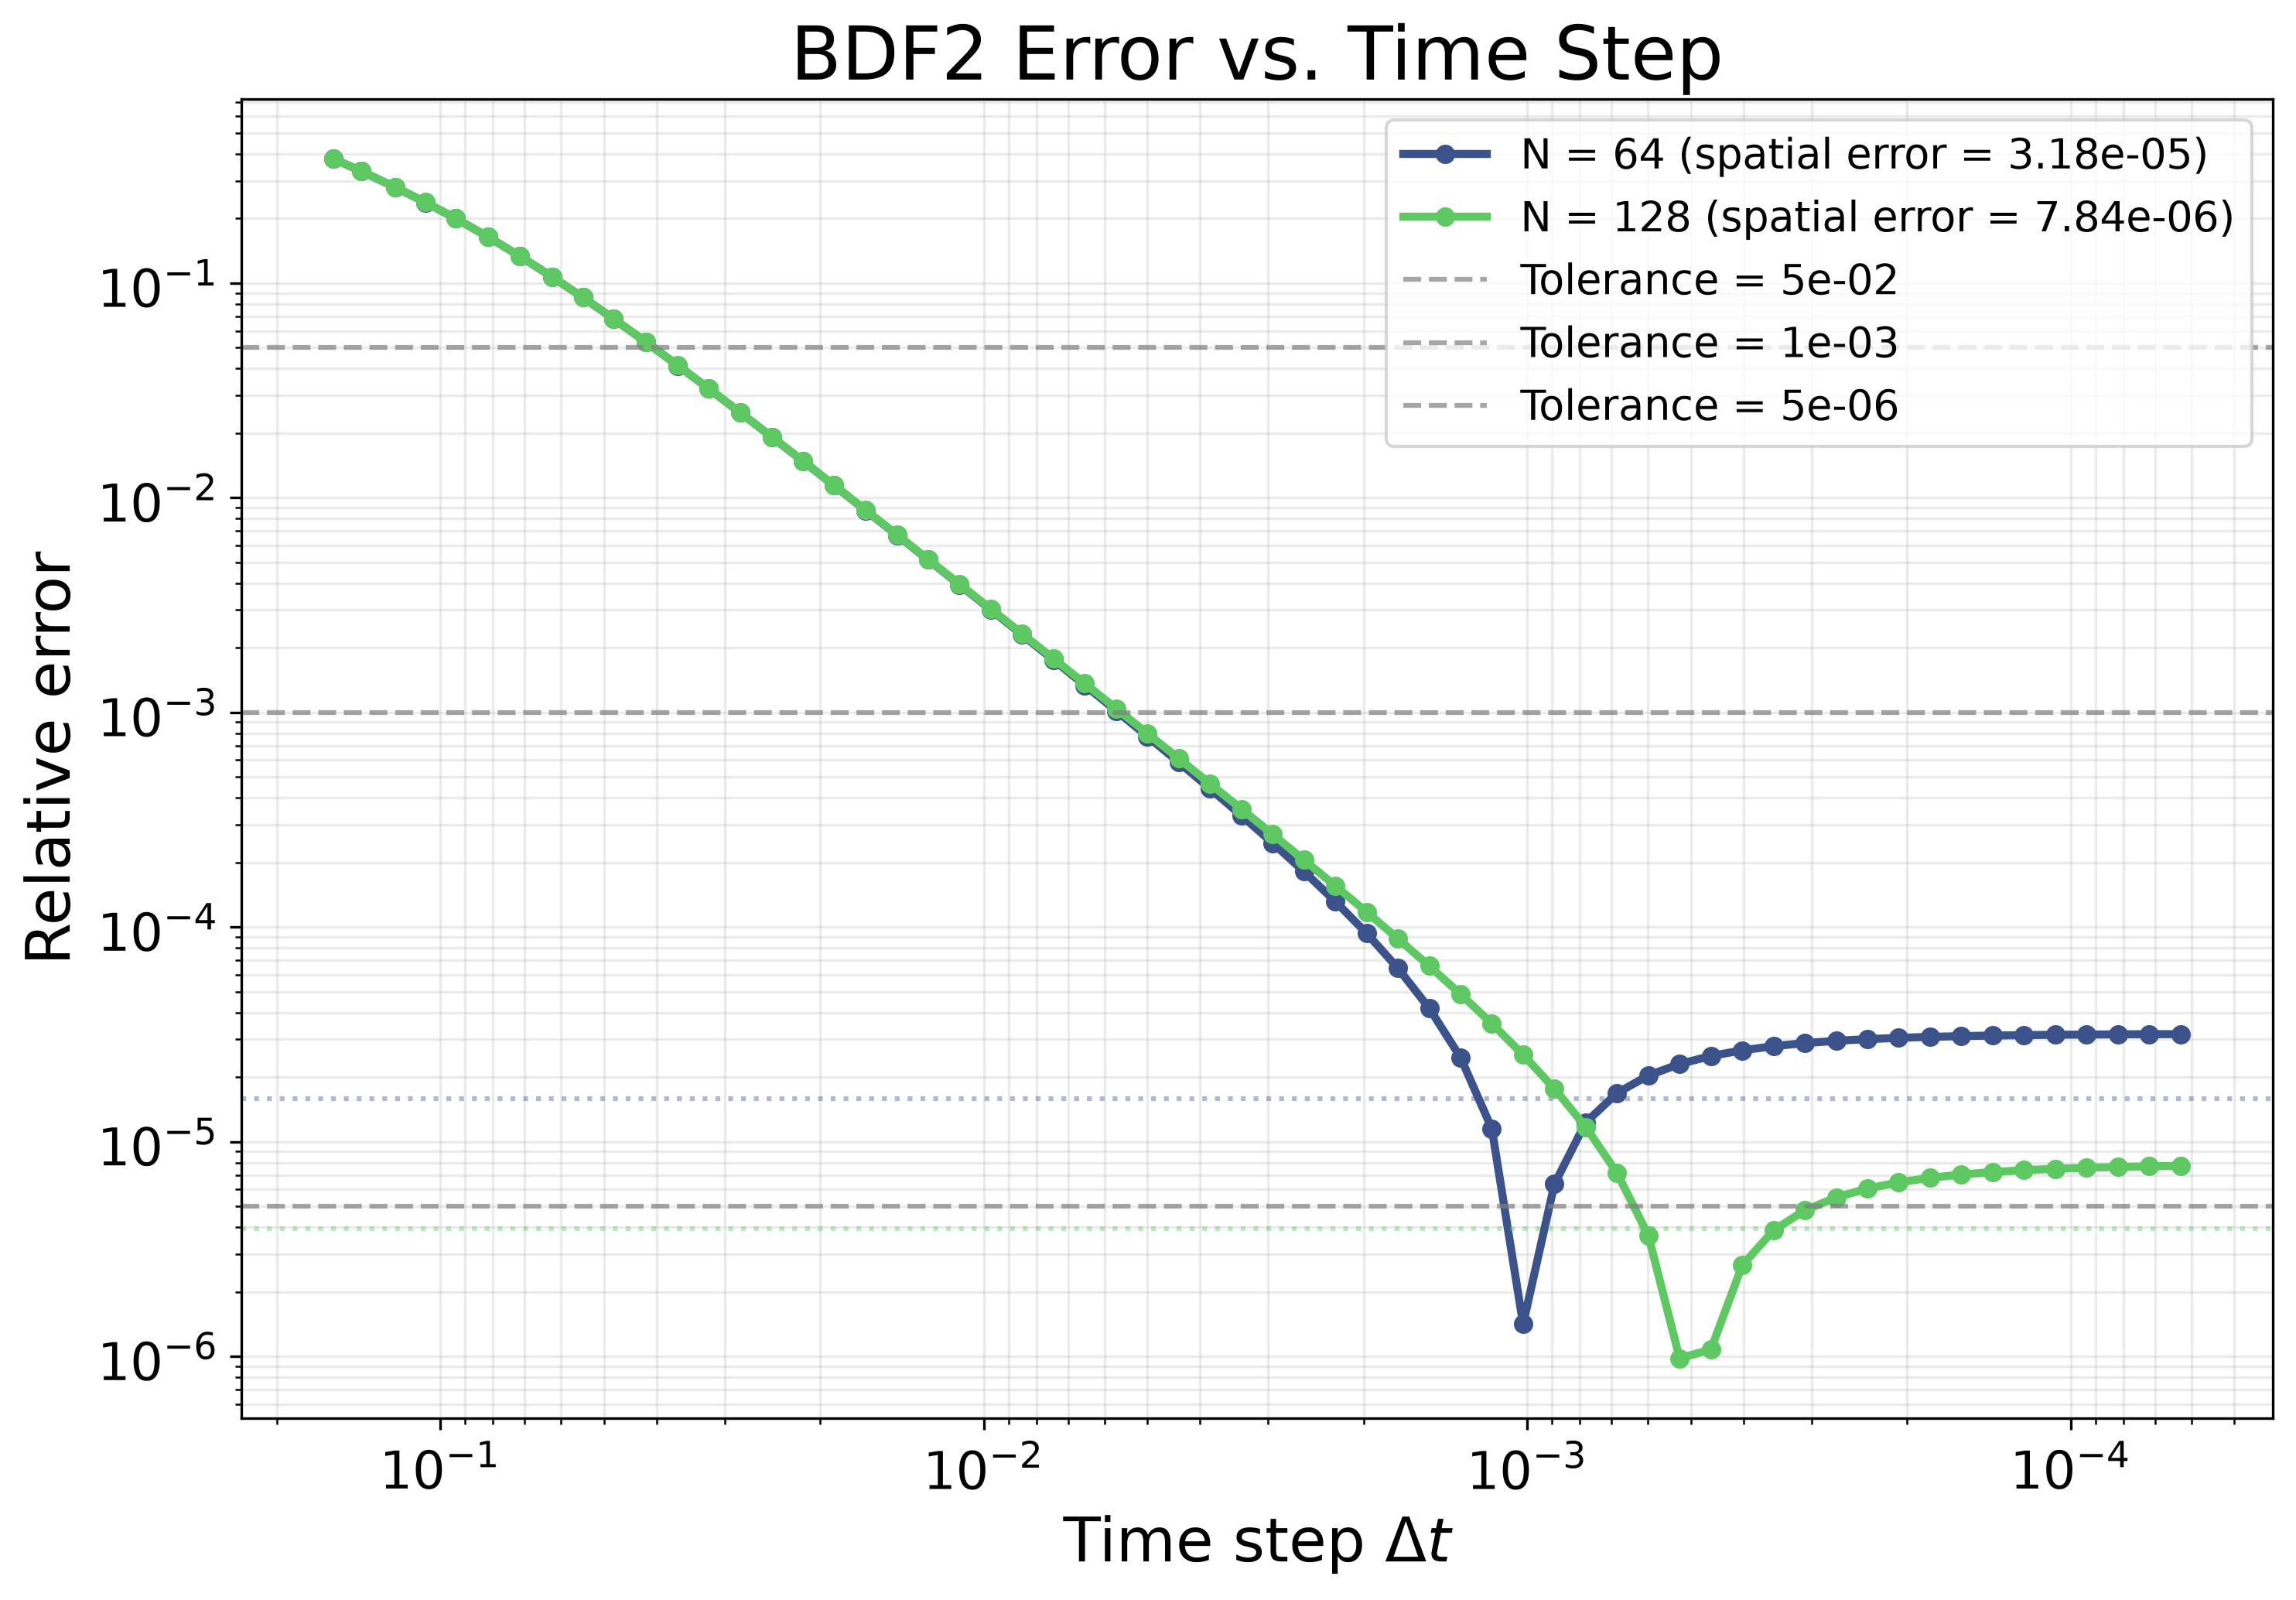
\includegraphics[width=0.8\textwidth]{problem2_BDF2.png}
\caption{BDF2 error and the three tolerances.}
\end{figure}

The FE and RK2 curves show the spatial-error plateau clearly. BE decreases slower, so its plateau is harder to see over the time steps plotted. CN and BDF2 have sharp dips where the time and spatial errors cancel each other out. Although the error falls below a tolerance, it can rise again for smaller $\Delta t$ because the spatial error dominates. 

I estimated the computational costs using $N^2$ spatial unknowns, with matrix-vector multiplication cost $O(N^2)$, sparse solve cost $O(N^2\log(N^2))$, and factorization cost $O(N^3)$. The resulting estimates are
\begin{align*}
 C_{\mathrm{FE}}&=5N^2s,\\
 C_{\mathrm{BE}}&=N^3+sN^2\log(N^2),\\
 C_{\mathrm{CN}}&=N^3+s\bigl(5N^2+N^2\log(N^2)\bigr),\\
 C_{\mathrm{RK2}}&=10N^2s,\\
 C_{\mathrm{BDF2}}&=2N^3+5N^2+sN^2\log(N^2),
\end{align*}
where $s=T/\Delta t$ is the number of time steps. 

\begin{table}[H]
\centering
\small
\begin{tabular}{cccccc}
\toprule
$N$ & Tolerance & Method & Steps & $\Delta t$ & Cost \\
\midrule
64 & $5\times10^{-2}$ & FE   & 2527  & $2.486\times10^{-3}$ & $5.175\times10^7$ \\
   &                   & BE   & 2     & $3.142$              & $3.303\times10^5$ \\
   &                   & CN   & 2     & $3.142$              & $3.712\times10^5$ \\
   &                   & RK2  & 2527  & $2.486\times10^{-3}$ & $1.035\times10^8$ \\
   &                   & BDF2 & 2     & $3.142$              & $6.129\times10^5$ \\
\midrule
64 & $1\times10^{-3}$ & FE   & 10108 & $6.216\times10^{-4}$ & $2.070\times10^8$ \\
   &           & BE   & 2     & $3.142$              & $3.303\times10^5$ \\
   &           & CN   & 2     & $3.142$              & $3.712\times10^5$ \\
   &           & RK2  & 2527  & $2.486\times10^{-3}$ & $1.035\times10^8$ \\
   &           & BDF2 & 2     & $3.142$              & $6.129\times10^5$ \\
\midrule
64 & $5\times10^{-6}$ & FE   & -- & -- & -- \\
   &                   & BE   & -- & -- & -- \\
   &                   & CN   & -- & -- & -- \\
   &                   & RK2  & -- & -- & -- \\
   &                   & BDF2 & -- & -- & -- \\
\midrule
128 & $5\times10^{-2}$ & FE   & 10269 & $6.119\times10^{-4}$ & $8.412\times10^8$ \\
    &                   & BE   & 2     & $3.142$              & $2.415\times10^6$ \\
    &                   & CN   & 2     & $3.142$              & $2.579\times10^6$ \\
    &                   & RK2  & 10269 & $6.119\times10^{-4}$ & $1.682\times10^9$ \\
    &                   & BDF2 & 2     & $3.142$              & $4.594\times10^6$ \\
\midrule
128 & $1\times10^{-3}$ & FE   & 10269 & $6.119\times10^{-4}$ & $8.412\times10^8$ \\
    &           & BE   & 2     & $3.142$              & $2.415\times10^6$ \\
    &           & CN   & 2     & $3.142$              & $2.579\times10^6$ \\
    &           & RK2  & 10269 & $6.119\times10^{-4}$ & $1.682\times10^9$ \\
    &           & BDF2 & 2     & $3.142$              & $4.594\times10^6$ \\
\midrule
128 & $5\times10^{-6}$ & FE   & --    & --                    & -- \\
    &                   & BE   & --    & --                    & -- \\
    &                   & CN   & 8192  & $7.670\times10^{-4}$ & $1.976\times10^9$ \\
    &                   & RK2  & --    & --                    & -- \\
    &                   & BDF2 & 16384 & $3.835\times10^{-4}$ & $2.609\times10^9$ \\
\bottomrule
\end{tabular}
\caption{Time steps and estimated computational costs for each method and tolerance. A dash indicates that the tolerance was not reached in the tested time steps.}
\end{table}

Backward Euler had the lowest computational cost for the two larger tolerances. FE and RK2 were more expensive because they required much smaller time steps to remain stable.

For the smallest tolerance, most methods did not reach the tolerance because the spatial error dominated. CN and BDF2 reached the tolerance for $N=128$, but this appears to be due to cancellation between spatial and temporal errors given the figures above. As a result, the error can increase again as $\Delta t$ decreases.

The time steps in the table are the first ones that satisfy each tolerance when doubling the number of steps, so they are not necessarily the largest possible time steps.

\newpage
\section*{Extra Credit: Adaptive RK45}
\textbf{Question.} Solve the same heat equation using an adaptive RK45 method and investigate how the time-step sizes change for $N=64$ and $N=128$.

\subsection*{Solution}
I used SciPy's \texttt{solve\_ivp} with the RK45 method to solve
\[
 \frac{d\mathbf{u}}{dt}=L\mathbf{u}+\mathbf{f}(t)
\]
from $t=0$ to $T=2\pi$. Unlike the previous methods, RK45 chooses its time-step sizes automatically. I used relative and absolute tolerances of $10^{-6}$ and $10^{-8}$, respectively.

I calculated the final relative error using the same formula as Problem 1. These solver tolerances control the time integration and do not remove the spatial discretization error.

\begin{figure}[H]
\centering
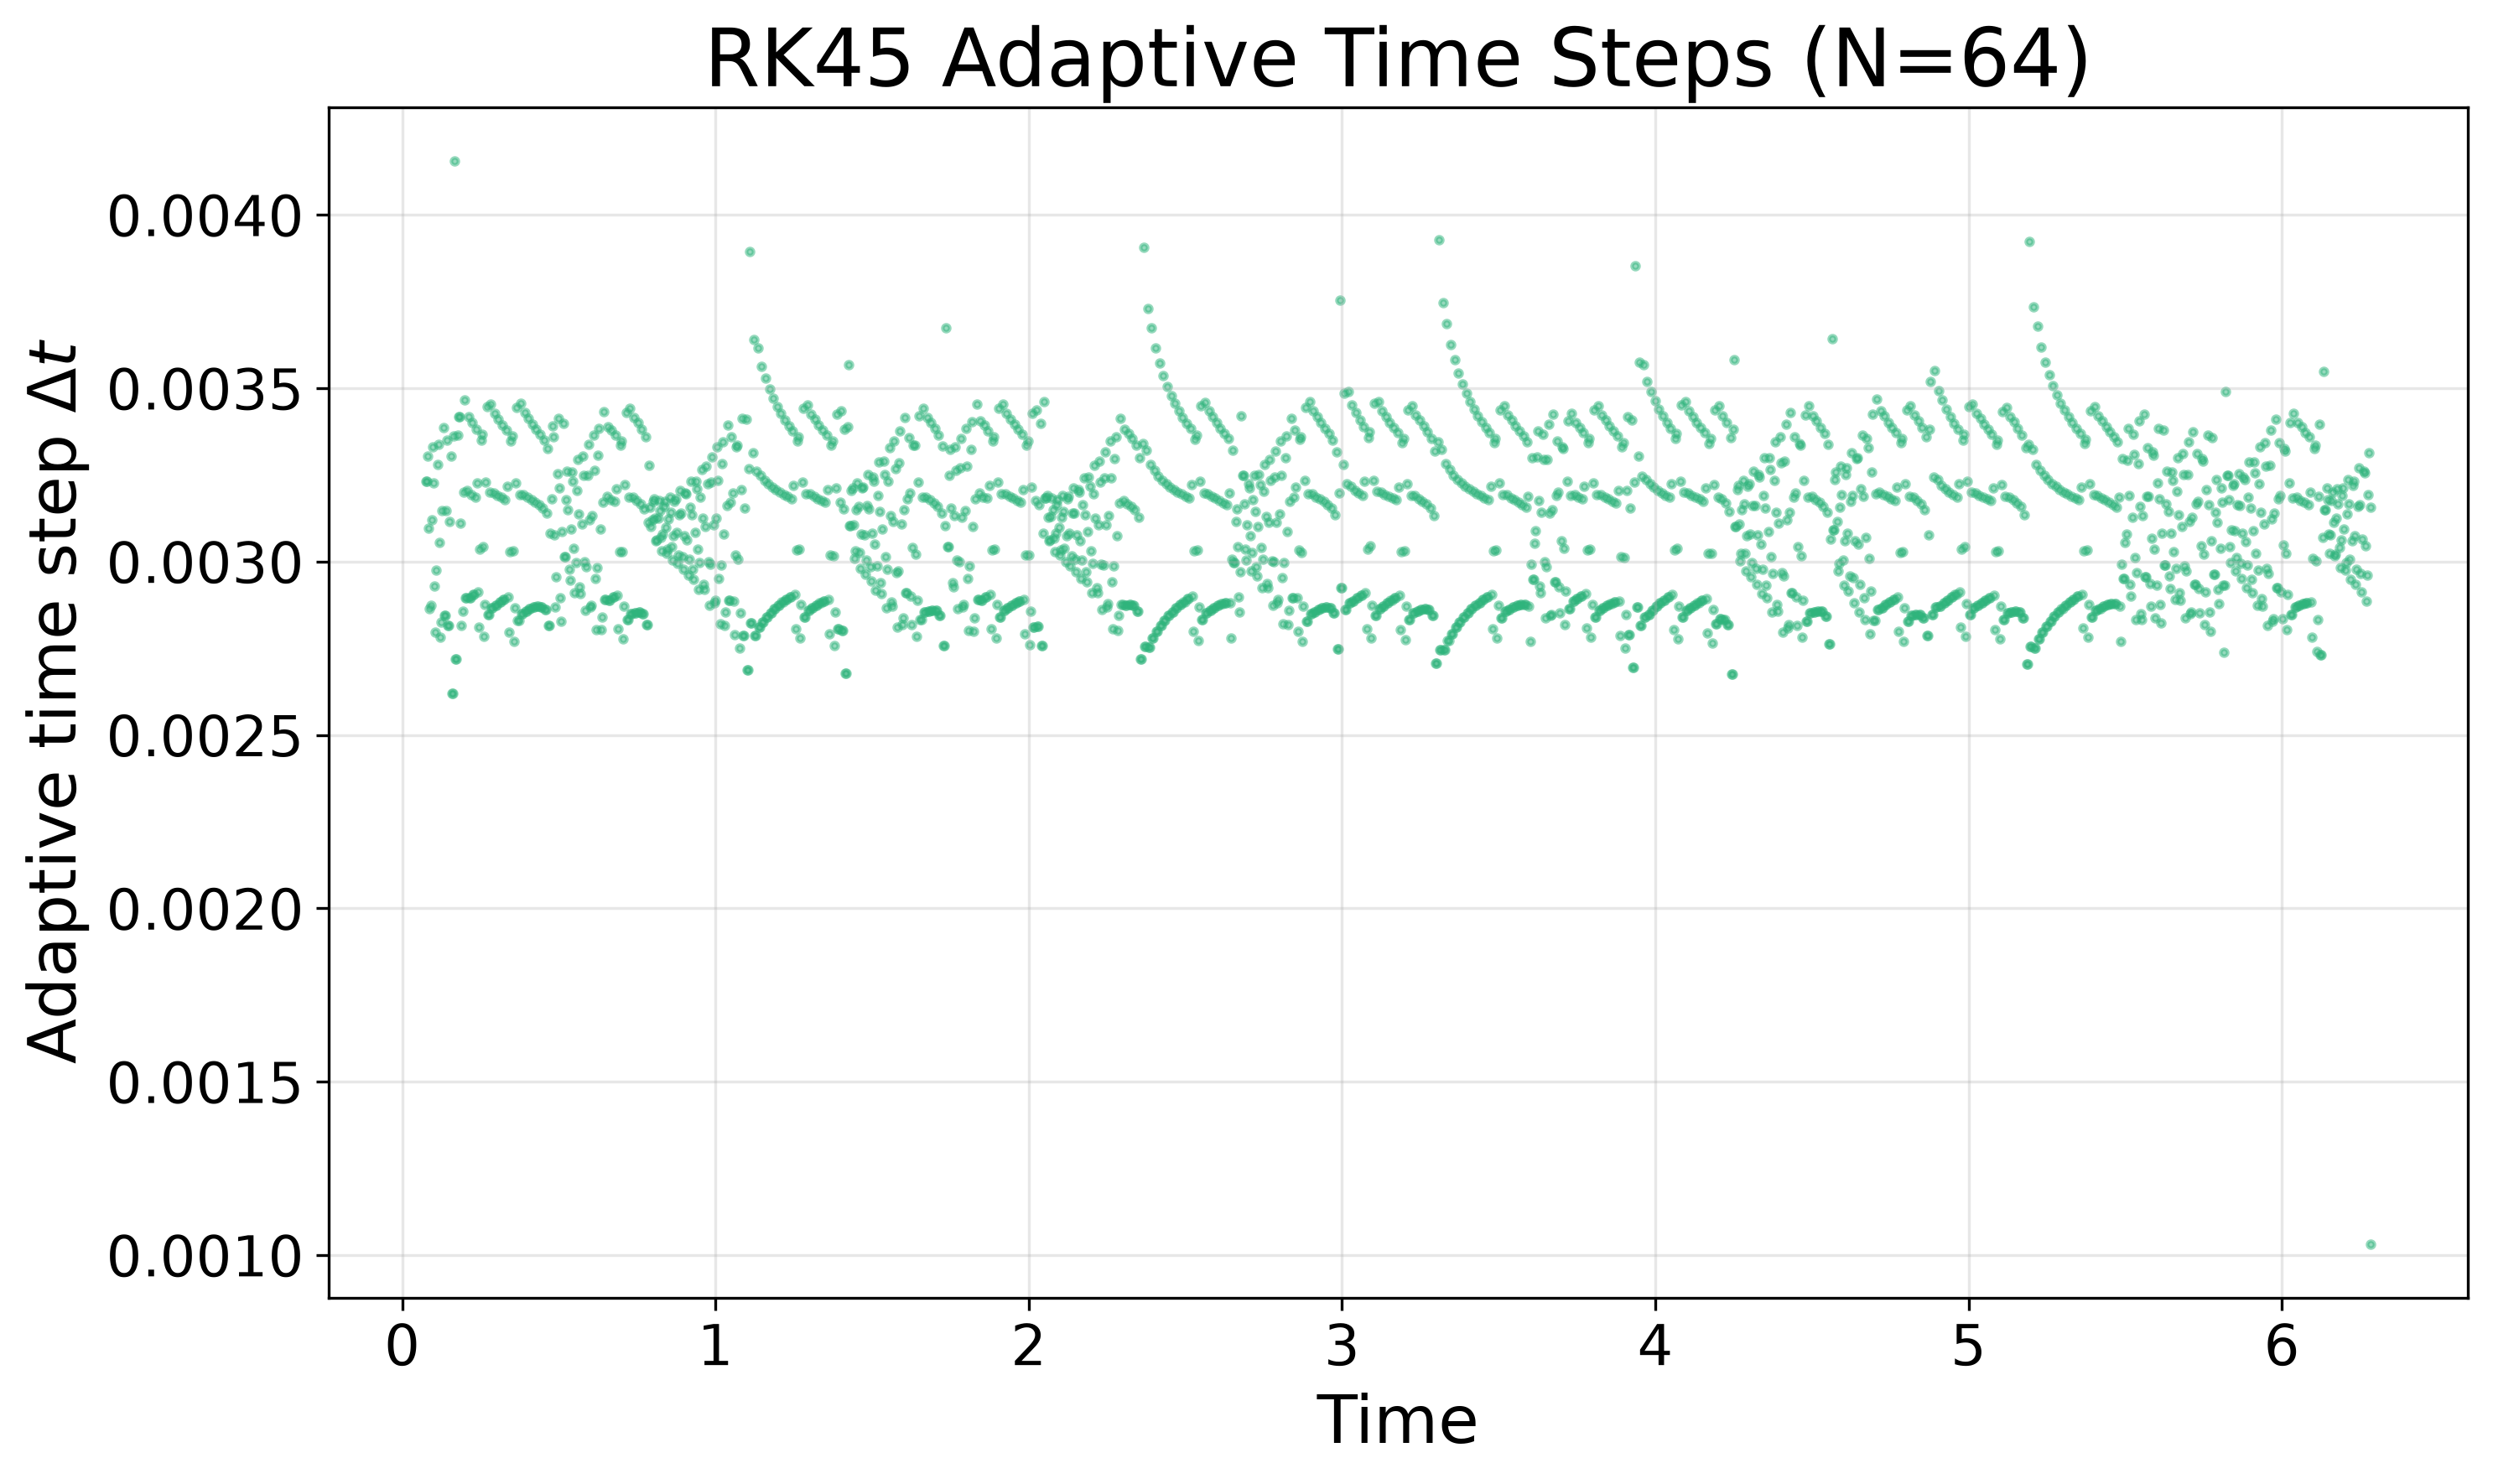
\includegraphics[width=0.78\textwidth]{RK45_steps_64.png}
\caption{Adaptive RK45 time steps for $N=64$.}
\end{figure}

\begin{figure}[H]
\centering
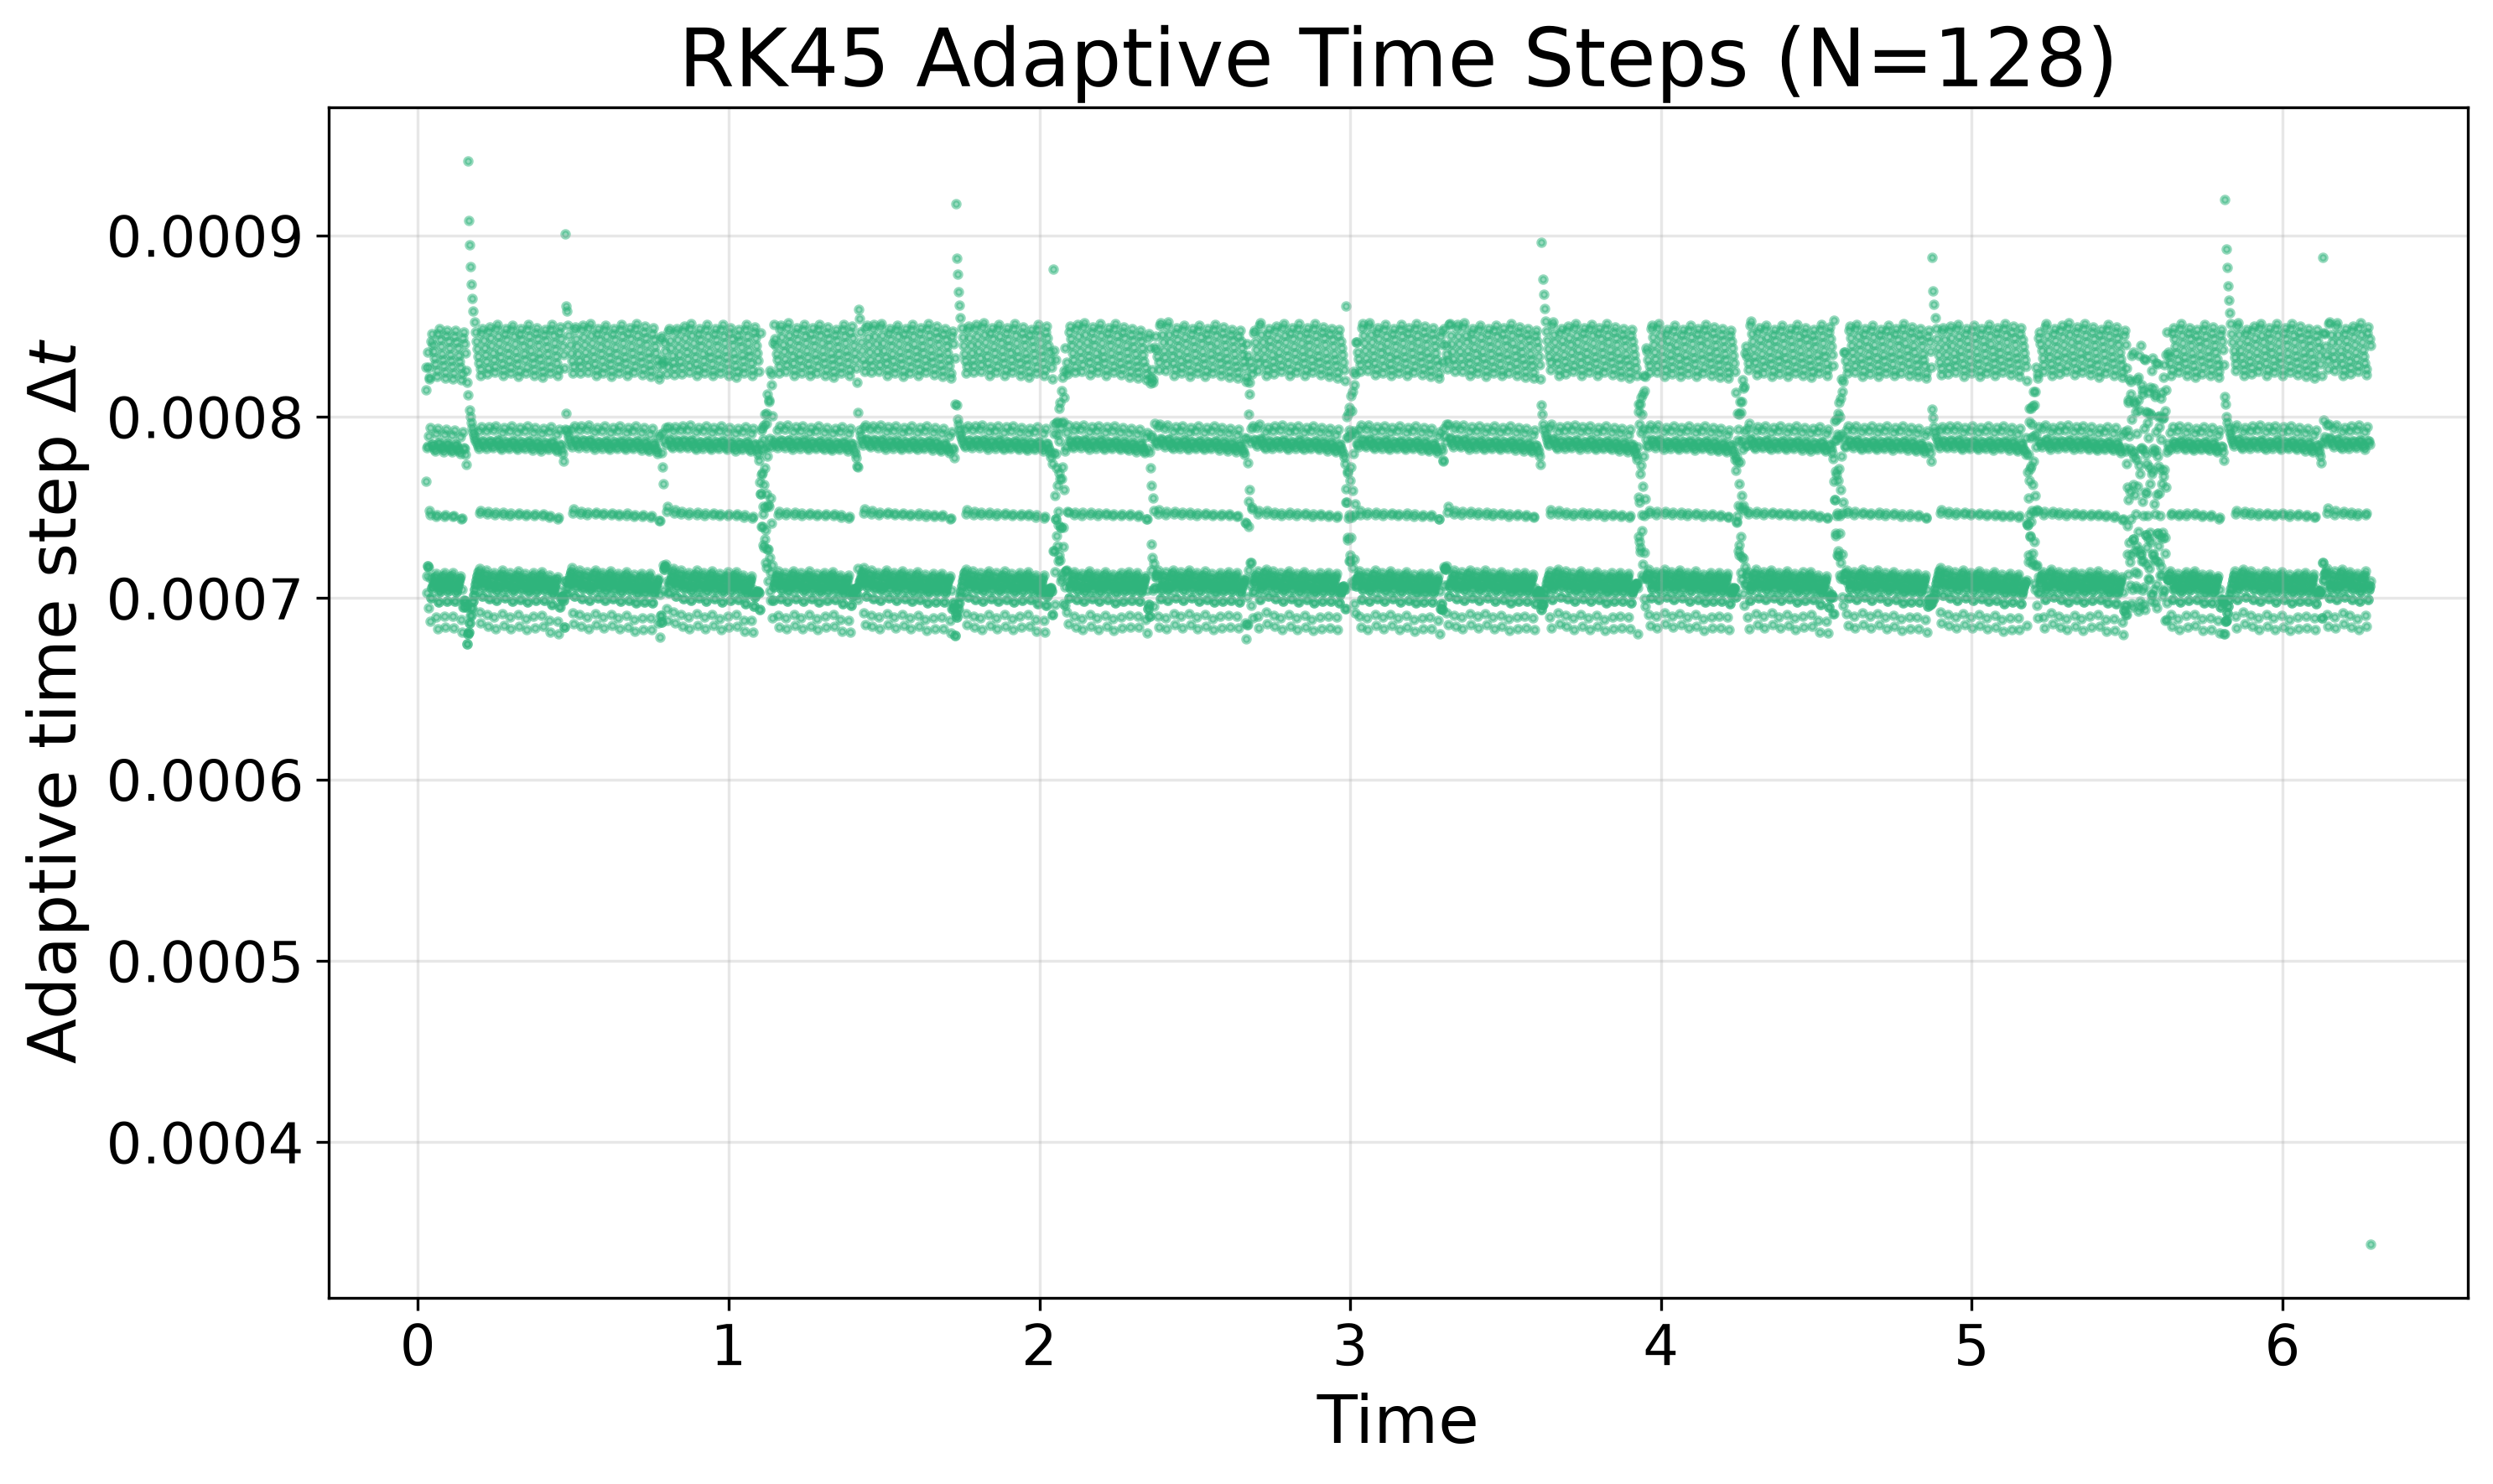
\includegraphics[width=0.78\textwidth]{RK45_steps_128.png}
\caption{Adaptive RK45 time steps for $N=128$.}
\end{figure}

For $N=64$, most time steps are around $0.003$, while for $N=128$ they are around $0.00075$. This is approximately a factor of four. The smaller spatial grid spacing makes the method's stability restriction more limiting. I thought it was interesting that RK45 still adjusts its time steps, but they stay within a fairly narrow range for most of the simulation. The final step is smaller because the solver has to end at exactly $T=2\pi$.

\end{document}